        %%******************************************%%
        %%                                          %%
        %%        Modello di tesi di laurea         %%
        %%            di Andrea Giraldin            %%
        %%                                          %%
        %%             2 novembre 2012              %%
        %%                                          %%
        %%******************************************%%

%**************************************************************
% file contenente le impostazioni della tesi
%**************************************************************


%**************************************************************
% Impostazioni di impaginazione
% see: http://wwwcdf.pd.infn.it/AppuntiLinux/a2547.htm
%**************************************************************

\setlength{\parindent}{14pt}   % larghezza rientro della prima riga
\setlength{\parskip}{0pt}   % distanza tra i paragrafi



%**************************************************************
% Impostazioni di biblatex
%**************************************************************
\bibliography{bibliografia} % database di biblatex 

\defbibheading{bibliography} {
    \cleardoublepage
    \phantomsection 
    \addcontentsline{toc}{chapter}{\bibname}
    \chapter*{\bibname\markboth{\bibname}{\bibname}}
}

\setlength\bibitemsep{1.5\itemsep} % spazio tra entry

\DeclareBibliographyCategory{opere}
\DeclareBibliographyCategory{web}

\addtocategory{opere}{womak:lean-thinking}
\addtocategory{web}{site:agile-manifesto}

\defbibheading{opere}{\section*{Riferimenti bibliografici}}
\defbibheading{web}{\section*{Siti Web consultati}}


%**************************************************************
% Impostazioni di caption
%**************************************************************
\captionsetup{
    tableposition=top,
    figureposition=bottom,
    font=small,
    format=hang,
    labelfont=bf
}

%**************************************************************
% Impostazioni di glossaries
%**************************************************************

%**************************************************************
% Acronimi
%**************************************************************
\renewcommand{\acronymname}{Acronimi e abbreviazioni}

%no acronimi e abbreviazioni

\iffalse
\newacronym[description={\glslink{apig}{Application Program Interface}}]
    {api}{API}{Application Program Interface}
\fi

%**************************************************************
% Glossario
%**************************************************************
%\renewcommand{\glossaryname}{Glossario}
\renewcommand{\glsnamefont}[1]{\makefirstuc{#1}}


%%%%%%%%%%%%%%%%%%%%%%%%%%%%%%%%%%%%%%%%%%%%%%%%%%%%%%%%%%%%%%%%%%%%%%%%%%%%

%no termini glossario
%tutto è definito subito in footnote

\iffalse
\newglossaryentry{asset}
{
    name=asset,
    sort=asset,
    description={todo}
}
\fi
 % database di termini
\makeglossaries


%**************************************************************
% Impostazioni di graphicx
%**************************************************************
\graphicspath{{immagini/}} % cartella dove sono riposte le immagini


%**************************************************************
% Impostazioni di hyperref
%**************************************************************
\hypersetup{
    %hyperfootnotes=false,
    %pdfpagelabels,
    %draft,	% = elimina tutti i link (utile per stampe in bianco e nero)
    colorlinks=true,
    linktocpage=true,
    pdfstartpage=1,
    pdfstartview=,
    % decommenta la riga seguente per avere link in nero (per esempio per la stampa in bianco e nero)
    %colorlinks=false, linktocpage=false, pdfborder={0 0 0}, pdfstartpage=1, pdfstartview=FitV,
    breaklinks=true,
    pdfpagemode=UseNone,
    pageanchor=true,
    pdfpagemode=UseOutlines,
    plainpages=false,
    bookmarksnumbered,
    bookmarksopen=true,
    bookmarksopenlevel=1,
    hypertexnames=true,
    pdfhighlight=/O,
    %nesting=true,
    %frenchlinks,
    urlcolor=webbrown,
    linkcolor=RoyalBlue,
    citecolor=webgreen,
    %pagecolor=RoyalBlue,
    %urlcolor=Black, linkcolor=Black, citecolor=Black, %pagecolor=Black,
    %pdftitle={\myTitle},
    %pdfauthor={\textcopyright\ \myName, \myUni, \myFaculty},
    %pdfsubject={},
    %pdfkeywords={},
    %pdfcreator={pdfLaTeX},
    %pdfproducer={LaTeX}
}

%**************************************************************
% Impostazioni di itemize
%**************************************************************
\renewcommand{\labelitemi}{$\bullet$}

%\renewcommand{\labelitemi}{$\bullet$}
%\renewcommand{\labelitemii}{$\cdot$}
%\renewcommand{\labelitemiii}{$\diamond$}
%\renewcommand{\labelitemiv}{$\ast$}


%**************************************************************
% Impostazioni di listings
%**************************************************************
\lstset{
    language=[LaTeX]Tex,%C++,
    keywordstyle=\color{RoyalBlue}, %\bfseries,
    basicstyle=\small\ttfamily,
    %identifierstyle=\color{NavyBlue},
    commentstyle=\color{Green}\ttfamily,
    stringstyle=\rmfamily,
    numbers=none, %left,%
    numberstyle=\scriptsize, %\tiny
    stepnumber=5,
    numbersep=8pt,
    showstringspaces=false,
    breaklines=true,
    frameround=ftff,
    frame=single
} 
\colorlet{punct}{red!60!black}
\definecolor{background}{HTML}{EEEEEE}
\definecolor{delim}{RGB}{20,105,176}
\colorlet{numb}{magenta!60!black}
\definecolor{codegreen}{rgb}{0,0.6,0}
\definecolor{codegray}{rgb}{0.5,0.5,0.5}
\definecolor{codepurple}{rgb}{0.82, 0.62, 0.91}
\definecolor{codeblue}{rgb}{0, 0.5, 1}
\definecolor{codeorange}{rgb}{1, 0.22, 0}

% Define the codebox
\lstdefinelanguage{dart}{
backgroundcolor=\color{background},   
    commentstyle=\color{codegreen},
    basicstyle=\ttfamily\footnotesize,
    breakatwhitespace=false,         
    breaklines=true, 
    stepnumber=1,
    captionpos=b,                    
    keepspaces=true,                 
    numbers=left,                    
    numbersep=8pt,                  
    showspaces=false,                
    showstringspaces=false,
    showtabs=false,                  
    tabsize=2,
    %frame=shadowbox
    emph=[1]{CheckLogin, HookWidget, Widget, BuildContext, bool, String, int, List, GenericErrorPage, LoginScreen, LoadUser, LoadCoach, DelayedWidget, Widget, Key, this, super, Future, false, true, Duration, Waiter, List, Goals, Appointment, ChangeNotifierProvider, UserRepo, Provider, ChangeNotifier, Reader, User, Options, Dio, Future },% Insert here the types you are using
    emphstyle=[1]{\color{codeblue}},
    emph=[2]{useProvider, build, useState, useEffect, delayed, then, buildCards, addAll, buildGoalsCards, where, map, toList, buildAppointmentCards, getAccessToken, fetchUser, watch, notifyListeners},% Insert here the methods you are using
    emphstyle=[2]{\color{codepurple}},
    emph=[3]{class, extends, @override, if, return, else, switch, case, default, final, required, is, as, =>, async, void, try, catch, finally, await},% Insert here the keywords you are using
    emphstyle=[3]{\color{codeorange}},%
}

\lstdefinelanguage{json}{
    basicstyle=\ttfamily\footnotesize,
    numbers=left,
    numberstyle=\scriptsize,
    stepnumber=1,
    numbersep=8pt,
    showstringspaces=false,
    breaklines=true,
    backgroundcolor=\color{background},
    string=[s]{"}{"},
    stringstyle=\color{blue},
    comment=[l]{:},
    commentstyle=\color{black},
    literate=
     *{0}{{{\color{numb}0}}}{1}
      {1}{{{\color{numb}1}}}{1}
      {2}{{{\color{numb}2}}}{1}
      {3}{{{\color{numb}3}}}{1}
      {4}{{{\color{numb}4}}}{1}
      {5}{{{\color{numb}5}}}{1}
      {6}{{{\color{numb}6}}}{1}
      {7}{{{\color{numb}7}}}{1}
      {8}{{{\color{numb}8}}}{1}
      {9}{{{\color{numb}9}}}{1}
      {:}{{{\color{punct}{:}}}}{1}
      {,}{{{\color{punct}{,}}}}{1}
      {[}{{{\color{delim}{[}}}}{1}
      {]}{{{\color{delim}{]}}}}{1},
}


%**************************************************************
% Impostazioni di xcolor
%**************************************************************
\definecolor{webgreen}{rgb}{0,.5,0}
\definecolor{webbrown}{rgb}{.6,0,0}


%**************************************************************
% Altro
%**************************************************************

\newcommand{\omissis}{[\dots\negthinspace]} % produce [...]

% eccezioni all'algoritmo di sillabazione
\hyphenation
{
    ma-cro-istru-zio-ne
    gi-ral-din
}

\newcommand{\sectionname}{sezione}
\addto\captionsitalian{\renewcommand{\figurename}{Figura}
                       \renewcommand{\tablename}{Tabella}}

\newcommand{\glsfirstoccur}{\ap{{[g]}}}

\newcommand{\intro}[1]{\emph{\textsf{#1}}}

%**************************************************************
% Environment per ``rischi''
%**************************************************************
\newcounter{riskcounter}                % define a counter
\setcounter{riskcounter}{0}             % set the counter to some initial value

%%%% Parameters
% #1: Title
\newenvironment{risk}[1]{
    \refstepcounter{riskcounter}        % increment counter
    \par \noindent                      % start new paragraph
    \textbf{\arabic{riskcounter}. #1}   % display the title before the 
                                        % content of the environment is displayed 
}{
    \par\medskip
}

\newcommand{\riskname}{Rischio}

\newcommand{\riskdescription}[1]{\textbf{\\Descrizione:} #1.}

\newcommand{\risksolution}[1]{\textbf{\\Soluzione:} #1.}

%**************************************************************
% Environment per ``use case''
%**************************************************************
\newcounter{usecasecounter}             % define a counter
\setcounter{usecasecounter}{0}          % set the counter to some initial value

%%%% Parameters
% #1: ID
% #2: Nome
\newenvironment{usecase}[2]{
    \renewcommand{\theusecasecounter}{\usecasename #1}  % this is where the display of 
                                                        % the counter is overwritten/modified
    \refstepcounter{usecasecounter}             % increment counter
    \vspace{10pt}
    \par \noindent                              % start new paragraph
    {\large \textbf{\usecasename #1: #2}}       % display the title before the 
                                                % content of the environment is displayed 
    \medskip
}{
    \medskip
}

\newcommand{\usecasename}{UC}

\newcommand{\usecaseactors}[1]{\textbf{\\Attori Principali:} #1. \vspace{4pt}}
\newcommand{\usecasepre}[1]{\textbf{\\Precondizioni:} #1. \vspace{4pt}}
\newcommand{\usecasedesc}[1]{\textbf{\\Descrizione:} #1. \vspace{4pt}}
\newcommand{\usecasepost}[1]{\textbf{\\Postcondizioni:} #1. \vspace{4pt}}
\newcommand{\usecasealt}[1]{\textbf{\\Scenario Alternativo:} #1. \vspace{4pt}}

%**************************************************************
% Environment per ``namespace description''
%**************************************************************

\newenvironment{namespacedesc}{
    \vspace{10pt}
    \par \noindent                              % start new paragraph
    \begin{description} 
}{
    \end{description}
    \medskip
}

\newcommand{\classdesc}[2]{\item[\textbf{#1:}] #2}
%**************************************************************
%cose mie
\definecolor{red}{cmyk}{0,0.87,0.68,0.32}
\newcolumntype{C}[1]{>{\centering\let\newline\\\arraybackslash\hspace{0pt}}m{#1}}

\newcommand{\vsc}{{Visual Studio Code}}
\newcommand{\astudio}{{Android Studio}}
%\newcommand{\flutter}{\textit{Flutter}} %nomi propri no corsivo
%\newcommand{\swift}{\textit{Swift}}
%\newcommand{\kotlin}{\textit{Kotlin}}
%\newcommand{\java}{\textit{Java}}
%\newcommand{\unity}{\textit{Unity}}
%\newcommand{\dart}{\textit{Dart}}
\newcommand{\arplug}{{ar\_flutter\_plugin}}
%\newcommand{\arcore}{\textit{ARCore}}
\newcommand{\aws}{Amazon Web Services}
\newcommand{\asa}{Azure Spatial Anchors}

\newcommand{\todo}{\textbf{\large{\textcolor{todoOrange}{TODO}}}}
%\newcommand{\E}{\`E} %maiuscole con apostrofo e non accento
\newcommand{\aCapo}{ ~ \vspace{0.22cm} \\} %magari fare renewcommand di paragraph 



\begin{document}
\pagecolor{blond}
%**************************************************************
% Materiale iniziale
%**************************************************************
\frontmatter
\input{inizio-fine/frontespizio}
\input{inizio-fine/colophon}
%\input{inizio-fine/dedica}
% !TEX encoding = UTF-8
% !TEX TS-program = pdflatex
% !TEX root = ../tesi.tex

%**************************************************************
% Sommario
%**************************************************************
\cleardoublepage
\phantomsection
\pdfbookmark{Sommario}{Sommario}
\begingroup
\let\clearpage\relax
\let\cleardoublepage\relax
\let\cleardoublepage\relax

\chapter*{Sommario}

Il presente documento è il resoconto della mia attività di tirocinio, della durata di circa trecentoventi ore, presso l'azienda Datasoil S.r.l.\\
L'obiettivo principale è stato la progettazione e l'implementazione di un'applicazione multipiattaforma legata al mondo del wellness/fitness a supporto della piattaforma di analisi dati realizzata per un prodotto spinoff dell'azienda. Il tutto con un focus sull'usabilità e l'engagement/gamification.\\
Il prodotto è stato sviluppato utilizzando Dart come linguaggio di programmazione e Flutter come framework. In questo modo è stato possibile scrivere un'unica applicazione che possa funzionare sia su dispositivi Android, sia su dispositivi iOS.

%\vfill
%
%\selectlanguage{english}
%\pdfbookmark{Abstract}{Abstract}
%\chapter*{Abstract}
%
%\selectlanguage{italian}

\endgroup			

\vfill


% !TEX encoding = UTF-8
% !TEX TS-program = pdflatex
% !TEX root = ../tesi.tex

%**************************************************************
% Ringraziamenti
%**************************************************************
\cleardoublepage
\phantomsection
\pdfbookmark{Ringraziamenti}{ringraziamenti}

\bigskip

\begingroup
\let\clearpage\relax
\let\cleardoublepage\relax
\let\cleardoublepage\relax

\chapter*{Ringraziamenti}

\noindent \textit{Innanzitutto, vorrei esprimere la mia gratitudine al Prof. Tullio Vardanega, relatore della mia tesi, per il supporto preciso e puntuale fornitomi durante l'intera durata dello stage e la conseguente stesura della tesi.}\\

\noindent \textit{Un ringraziamento va ad Andrea e Pietro, riferimenti aziendali, e in generale a tutto il team Datasoil S.r.l. che mi ha permesso di vivere un'esperienza arricchente in un ambiente lavorativo sereno.}\\

\noindent \textit{Desidero infine ringraziare i miei familiari senza i quali mai avrei potuto intraprendere un percorso impegnativo come un corso di laurea.}\\


\bigskip

\noindent\textit{\myLocation, \myTime}
\hfill \myName

\endgroup


\input{inizio-fine/indici}
\cleardoublepage

%**************************************************************
% Materiale principale
%**************************************************************
\mainmatter
% !TEX encoding = UTF-8
% !TEX TS-program = pdflatex
% !TEX root = ../tesi.tex

%**************************************************************
\chapter{Contesto Aziendale}
\label{cap:contesto-aziendale}
%**************************************************************

\section{L'azienda}
\subsection{Descrizione}
Le informazioni a seguito sono state prese direttamente dall'azienda, tuttavia ritengono siano rappresentative della realtà considerando sia il progetto al quale ho partecipato, sia il resto dell'offerta \textit{software}.\\
\textbf{Datasoil S.r.l.} è una \textit{startup} innovativa che si occupa di sviluppare applicativi dedicati alla gestione aziendale, altamente integrati con industria 4.0 e \textit{digital twin}: vengono impiegati \textit{machine learning} e analisi predittive per ottenere analitiche migliori rispetto alla concorrenza, con un occhio attento a innovazione, sicurezza e scalabilità, ottenute tramite prototipazione e \textit{Infrastrucutre as Code}, delegando quindi la gestione delle componenti \textit{server} a servizi terzi come \aws{} (ecosistema \textit{software} fornito da Amazon, che va da semplici piattaforme di \textit{cloud storage} fino a sistemi predittivi basati su \textit{machine learning}).\\
Il loro obiettivo è manipolare ed elaborare dati di natura inerentemente caotica, ordinarli e presentarli all'utente finale tramite interfacce grafiche intuitive, promuovendo un'interazione efficace tra utilizzatore e mezzo. Prediligono un approccio ai problemi condiviso e modulare per far nascere soluzioni inedite da applicare a grandi progetti, forti di un \textit{know-how} che abbraccia esigenze verticali (vengono impiegate internamente molte tecnologie sia lato \textit{frontend} che lato \textit{backend}).\\
Le piattaforme dedicate ad \textit{industry} 4.0, \textit{smart building} e \textit{smart city} poggiano su dei \textit{data silos} attualmente esistenti, garantendo un'interpretazione integrata e di alto livello delle informazioni aziendali fondendole con eventi provenienti dai diversi \textit{business level} creando \textit{insight} proattivi in tempo reale. I sistemi predittivi di Datasoil sono in grado di notificare la persona giusta al momento giusto anticipando la gestione delle criticità interfunzionali.\\
Ho avuto modo di verificare molte di queste affermazioni direttamente tramite il progetto proposto, in quanto si tratta di un applicativo legato all'industria 4.0 che mappa \textit{asset} aziendali (come ad esempio macchinari) ad un gemello digitale, permettendo sia di localizzarli su una mappa tridimensionale sia, obiettivo dello stage, di visualizzarli in realtà aumentata.\\

\subsection{Clientela}
Datasoil sviluppa applicazioni che guardano al mondo professionale più che a quello generico \textit{consumer}, ad esempio in questo specifico caso l'applicativo (che prende il nome di MobileSYN) è dedicato a un'utenza strettamente aziendale, e ci si aspetta che venga utilizzata da operatori interni con dispositivi controllati (generalmente \textit{tablet} Apple). \\
Anche un altro prodotto dell'azienda, chiamato LifestyleSync, mira a fornire uno strumento per migliorare il benessere dei dipendenti nelle aziende, permettendo a ogni dipendente di essere seguito da un \textit{coach} che, tramite un'applicazione di supporto LSCoach, può progettare allenamenti personalizzati e vedere la progressione degli stessi.

\subsection{Processi Interni}

\subsection{Innovazione}
%************************************************************************************************************
\section{Tecnologie e Strumenti}
\label{sec:tecnologie-e-strumenti}

\subsection{Tecnologie e Strumenti di sviluppo}
\subsubsection{Visual Studio Code}
\vsc{} è un editor per codice sorgente, sviluppato da \textit{Microsoft} servendosi del framework \textit{Electron}, disponibile per Windows, Linux e macOS. Le sue funzionalità comprendo supporto per debugging, syntax highlighting, intelligent code completion, snippets, code refactoring, e integrazione con Git. \\
Gli utenti possono configurare tema, macro, preferenze e installare estensioni che ne aumentano le funzionalità aggiungendo ad esempio il supporto ai maggiori linguaggi di porgrammazione attualmente presenti.\\
Nella \textit{Stack Overflow 2021 Developer Survey}, \vsc{} è risultato essere l'IDE più popolare, adottato dal 70\% degli intervistati. {\tiny Fonte: \href{https://en.wikipedia.org/wiki/Visual_Studio_Code}{Wikipedia}}\\
\E{} inoltre presente e molto comoda l'estensione di \flutter{} che, tra le altre cose, permette di gestire direttamente in gui i vari dispositivi (smartphone, browser o emulatore) sui quali installare e lanciare l'app che si sta programmando.

\subsubsection{Android Studio}
\textit{Android Studio} è l'IDE ufficiale del sistema operativo di Gooogle, sostituendo Eclipse dal 2015, costruito sul software IntelliJ di JetBrains e progettato specificatamente per lo sviluppo Android. \E{} disponibile per Windows, Linux e macOS.\\
Il 7 maggio 2019 Kotlin rimpiazzò Java come linguaggio consigliato per Android, favorendo un'integrazione ancora maggiore con JetBrains che, appunto, ha sviluppato e prodotto Kotlin stesso. {\tiny Fonte: \href{https://en.wikipedia.org/wiki/Android_Studio}{Wikipedia}}\\
Personalmente ho cercato nonostante tutto di programmare il più possibile su \vsc{} preferendolo quindi ad \textit{Android Studio} in virtù della sua maggiore leggerezza e delle sue più ampie possibilità di personalizzazione.

\subsubsection{Dart}
Dart è un linguaggio di programmazione sviluppato da Google per il client development, ovvero per web e mobile app, e può anche essere impiegato per la costruzione di applicazione desktop e server.\\
\E{} un linguaggio object-oriented, class-based, garbage-collected, strongly-typed e con una sintassi nello stile di C. Può compilare sia codice macchina che JavaScript e supporta interefacce, mixins, classi astratte, refined generics e type inference.{\tiny Fonte: \href{https://en.wikipedia.org/wiki/Dart_(programming_language)}{Wikipedia}}\\
Personalmente l'ho trovato elegante e conciso nella sua struttura, e presenta dei vantaggi consistenti come la null protection e le espressioni ternarie.

\subsubsection{Flutter}
Flutter è un framework open-source creato da Google per lo sviluppo della UI di applicazioni cross-platform per Android, iOS, Linux, macOS, Windows, Google Fuchsia e il web partendo da un singolo codebase.\\
Rialsciato a maggio 2017, le applicazioni in Flutter sono scritte in Dart e sfruttano molte delle features avanzate del linguaggio, e le componenti principali del framework sono:
\begin{itemize}
    \item \textbf{Dart platform:} Flutter gira all'interno della Dart Virtual Machine, che si serve di un execution engine just-in-time;
    \item \textbf{Flutter engine:} scritto primariamente in C++, fornisce supporto a basso livello per il rendering e implementa accessibilità, file e network I/O, supporto nativo per i plugin e molto altro;
    \item \textbf{Foundation library:} scritta in Dart, fornisce classi e funzioni di base che vengono usate per costruire gli applcativi in Flutter, come ad esempio le API per la comunicazione con l'engine;
    \item \textbf{Design-specific widgets:} Flutter contiene due famiglie di widget che si conformano a delle specifiche scuole di design: \textit{Material} per Google e \textit{Cupertino} per Apple;
    \item \textbf{Flutter DevTools:} famiglia di tools generici che vengono sfruttati per lo sviluppo di software in Flutter.
\end{itemize}
~\\
Inoltre, una libreria fondamentale per semplificare l'utilizzo di Flutter è \textit{Flutter Hooks}: lo scopo è implementare delle strutture simili agli Hooks di React, consentono di sostituire gli Stateful Widget riducendo il boilerplate code e semplificando la gestione di side-effect e ciclo di vita dei widget grazie alla funzione \textit{useEffect}.

\subsubsection{Java}
Java è un linguaggio di programmazione ad alto livello object-oriented progettato per avere il minor numero possibile di dipendenze implementative (favorendo quindi l'uso di interfacce e classi astratte) e, soprattutto, per aderire al motto \textit{"write once, run anywhere"}: il bytecode di Java può infatti girare senza necessità di ricompilazione su qualsiasi piattaforma che supporti la Java Virtual Machine (comunemente abbreviata in JVM).\\  
La sintassi è simile a quelle di C o C++, ma fornisce funzionalità dinamiche generalmente inedite per i linguaggi compilati, come reflection e modifica del codice a runtime.\\
Originalmente rilasciato nel 1995 come componente centrale della piattaforma Java per Sun Microsystems e sotto licenza proprietaria, dal 2007 la maggior parte dei suoi componenti sono diventati open-source sotto l'ombrello della \textit{GPL-2.0-only} (licenza specifica per software libero pubblicata dalla Free Software Foundation).\\
Sebbene Oracle (attuale proprietario di Sun Microsystems) offra un'implementazione proprietaria chiamata \textit{HotSpot JVM}, la specifica ufficiale è la \textit{OpenJDK JVM} che è gratuita, open-source e di default nella maggior parte delle distribuzioni Linux.

\subsubsection{Kotlin}
Kotlin è un linguaggio di programmazione cross-platform, staticamente tipizzato, progettato per avere completa interoperabilità con Java, gode di una sintassi più concisa di quest'ultimo grazie alla type inference di cui è dotato e dipende dalla \textit{Java Class Library} per la versione della JVM da usare.\\
\E{} inoltre in grado di compilare codice in JavaScript (sfruttato poi da applicazioni frontend) o codice nativo tramite \textit{LLVM} (per app iOS che condividono la business logic con applicazioni Android).\\
Incluso in Android Studio come alternativa al compilatore standard Java dal 2017, produce bytecode Java 8 di default ma permette al programmatore di scegliere delle versioni target successive (fino a Java 18).

\subsubsection{Azure Spatial Anchors}
Azure Spatial Anchors è un servizio di Microsoft mirato a fornire strumenti per sviluppare applicazioni in realtà aumentata su dispositivi iOS o Android predisposti per, rispettivamente, ARKit e ARCore, oppure su Microsoft HoloLens.\\
Permette di riconoscere spazi tridimensionali all'interno dei quali posizionare punti di interesse, chiamati Spatial Anchors, che possono essere salvati in cloud e poi recuperati, e possono essere messi in relazione a oggetti reali (come macchinari in un contesto industriale) o virtuali.

\subsubsection{ARCore}
ARCore, conosciuto anche come Google Play Services per AR, è un software development kit prodotto da Google per permettere lo sviluppo di applicazioni in realtà aumentata.\\
Si serve di tre componenti principali:
\begin{itemize}
    \item \textbf{6DOF:} il dispositivo sfrutta una piattaforma inerziale a sei assi per comprendere e tracciare la propria posizione relativa allo spazio;
    \item \textbf{Environmental understanding:} permette riconoscere dimensioni e locazione delle superfici lisce;
    \item \textbf{Light estimation:} permette al telefono di stimare le condizioni di luce dell'ambiente.
\end{itemize}
asa si appoggia proprio ad ARCore per implementare le proprie funzionalità di AR su Android.

\todo
\textcolor{todoOrange}{ar flutter plugin, sceneform?}


%**************************************************************
\subsection{Strumenti organizzativi}

\subsubsection{Slack}
Slack è una piattaforma di comunicazione istantanea di proprietà di Salesforce e sviluppata da Slack Technologies per Windows, Linux, macOS, Android e iOS.\\
Permette di comunicare tramite messaggi, chiamate vocali e video, e di inviare media e files nelle chat private o nei canali. Quest'ultimi fungono da aggregatori e permettono di suddividere tematicamente la comunicazione.\\
\E{} inoltre possibile suddividere a un livello ancora più alto tramite i \textit{workspaces}, che aggregano al proprio interno utenti, canali e applicazioni: sono proprio quest'ultime che mostrano con maggiore chiarezza l'orientamento \textit{corporate} di Slack, infatti fornisce integrazione nativa con i maggiori software gestionali e organizzativi (come ad esempio Jira, Zoom, Drive, Outlook, etc).

\subsubsection{Github}
GitHub è il più grande servizio di hosting di codice sorgente al mondo, abitualmente usato per sviluppare progetti open source, e fornisce vari servizi: version control di Git distribuito e access control, bug tracking, issue tracking, richieste di modifiche software, task management, integrazione continua e wiki per ogni progetto.\\ 
Permette inoltre, tramite forking, pull request e commenti, il miglioramento collaborativo del software, ad esempio risolvendo bug, aggiungendo funzionalità o migliorando quelle presenti.


% !TEX encoding = UTF-8
% !TEX TS-program = pdflatex
% !TEX root = ../tesi.tex

%**************************************************************
\chapter{Lo Stage}
\label{cap:lo-stage}
%**************************************************************
\section{Descrizione e temi}
Il progetto proposto prevede l'implementazione di una vista in realtà aumentata\footnote{Schermata che mostra il \textit{feed} della fotocamera e permette di interagirci come fosse uno spazio 3D renderizzato} per l'applicazione di ticketing e monitoraggio aziendale "\textbf{MobileSYN}".\\
Questo applicativo permette di creare un gemello digitale di un asset aziendale e posizionarlo all'interno di uno spazio virtuale tridimensionale, così da rendere visivamente più chiaro quali macchinari di un dato stabilimento industriale abbiano necessità di manutenzione (mediante apertura di ticket appositi).\\
Un ticket è semplicemente una notifica relativa ad un asset (perdita d'olio per un macchinario, carta esaurita per una stampante, etc) ma può anche essere libero da questo vincolo e trovarsi, in autonomia, posizionato nello spazio (ad esempio per segnalare una crepa su un muro).

\begin{figure}[ht]
    \centering
    \includegraphics[height=5cm]{plant_asset_screenshot}
    \caption{Asset "Compressor Intake" in stabilimento "Plant 1"}
\end{figure}

Tutte le funzionalità in realtà aumentata dovranno necessariamente appoggiarsi al servizio di \asa{} perchè i gemelli digitali già presenti nel sistema sfruttano proprio questa tecnologia per la propria localizzazione spaziale e, vista la natura multipiattaforma dell'applicazione, dovranno essere implementate sia in Android che in iOS.
Dalla vista dovrà essere possibile interagire con gli \textit{asset} e i \textit{ticket}, (posizionamento ed eliminazione in \textit{augmented reality}) provocando l'apparizione di una \textit{card} all' \textit{on-tap} dell'\textit{anchor}\footnote{Traducibile in italiano con il termine "angoraggio" è un punto di interesse in uno spazio tridimensionale, ovvero un punto che possiede delle coordinate \textit{(x,y,z)}, al quale possono essere collegati \textit{asset}, \textit{ticket} o altri ancoraggi.}, ovvero mostrando a schermo tramite una piccola finestra in sovraimpressione i vari ticket relativi all'\textit{asset} dopo che questo viene toccato, permettendo anche la visione del dettaglio o la rimozione dello stesso.

\begin{figure}[ht]
    \centering
    \includegraphics[height=5cm]{asset_card}
    \caption{\textit{Card} (in primo piano) relativa a una \textit{anchor} (in secondo piano) in vista in realtà aumentata}
\end{figure}

Per portare a termine gli obiettivi prefissati sarà necessario studiare dei \textit{framework}, dei \textit{plugin} o dei \sdk{} che permettono l'integrazione del codice nativo di \asa{} (che sarà Java per Android e Swift per iOS) con il \textit{framework} Flutter e il linguaggio su cui si poggia, ovvero Dart. 

\section{Strategia aziendale}
Da un punto di vista strettamente aziendale questo \textit{stage} è stato inquadrato in una strategia che prevede l'espansione di funzionalità per applicativi esistenti nell'ottica di fornire valore aggiunto ai clienti attuali e futuri: precedentemente a questo progetto non era presente alcuna componente in realtà aumentata in MobileSYN, mentre la strategia futura è un continuo miglioramento di ciò che è stato aggiunto. Infatti non sono state sufficienti otto settimane per ottenre un risultato professionalmente soddisfacente, e Datasoil nel futuro si occuperà di limare l'interfaccia grafica (anche osservando sul campo le abitudini d'uso della stessa da parte degli operatori) e migliorare pulizia ed efficienza del codice prodotto.\\
L'azienda si rapporta con gli \textit{stage} in un'ottica produttiva: si tratta spesso di attività che si innestano in lavori già in atto o che sarebbero comunqui stati eseguiti, tuttavia nel mio caso questo si è legato fortemente al concetto di innnovazione per la natura stessa del progetto che tratta, come già discusso, tematiche non comuni (nello specifico la realtà aumentata). L'azienda inoltre sfrutta gli \textit{stage} per effettuare un primo \textit{screening} per eventuali collaboratori da assumere.\\
L'azienda si è attivamente impiegata a supportare il mio \textit{stage} con tuttua una serie di attività: sono stato direttamente ospitato in azienda e ho avuto accesso a risorse aziendali (\textit{account} \aws{} per accedere a MobileSYN) e credenziali \asa{}, inoltre sia il \textit{junior} che il \textit{senior developer} di Datasoil che si occupano del lato \textit{frontend} mi hanno attivamente affiancato durante lo sviluppo nella fase di codifica. Ho inoltre ricevuto supporto nella fase di analisi dei requisiti e in altri piccoli problemi relativi alla configurazione dei dispositivi e dei programmi necessari ad affrontare lo \textit{stage}.

\section{Obiettivi}
\begin{itemize}
    \item Minimi:
        \begin{itemize}
            \item Studio e comprensione del linguaggio di programmazione Dart e del \textit{framework} Flutter;
            \item Analisi strumenti Azure: Azure Console e \asa{};
            \item Ricerca di \textit{framework} e \sdk{} per implementare le \asa{} in Flutter;
            \item Eventuale studio di linguaggi necessari alle implementazioni native, come ad esempio Kotlin, Java, Unity o Swift;
            \item Completamento del \textit{framework} scelto nell'app Flutter esistente;
            \item Completamento dello sviluppo dei componenti per rappresentare le \textit{anchor} nello spazio in realtà aumentata;
            \item Completamento dello sviluppo delle \api{} per l'interazione utente con gli ancoraggi in realtà aumentata;
        \end{itemize}
    \item Massimi: 
        \begin{itemize}
            \item Sviluppo di componenti per mappare \textit{asset} aziendali ad \textit{anchor};
            \item Sviluppo di componenti grafici per la visualizzazione di metriche e informazioni di controllo.
        \end{itemize}
\end{itemize}

\section{Vincoli}
Come precedentemente accennato, i vincoli in questo progetto sono due: 
\begin{itemize}
    \item Utilizzare Flutter come \textit{framework} sul quale implementare le componenti in realtà aumentata;
    \item La tecnologia scelta per gestire gli ancoraggi in realtà aumentata deve essere \asa{}.
\end{itemize}
Eccezion fatta per queste specifiche tecnologiche il resto è stato lasciato a mia discrezione personale, sebbene siano stati consigliati degli strumenti di sviluppo (\vsc{} e \astudio{} come \ide{}). 
Vincoli non tecnologici ma organizzativi sono da identificare nell'uso di Slack di GitHub: il primo usato per la comnicazione interna con i membri di dell'azienda, il secondo invece è il \textit{repository}\footnote{Spesso abbreviato con \textit{"repo"} è un generico archivio di codice sorgente e pacchetti \textit{software}. Spesso contiene anche \textit{metadata} e guide per la configurazione, uso ed estensione del codice che contiene. In genere un \textit{repo} ha una qualche forma di controllo di versione integrato.} dove si trova il codice sorgente di MobileSYN.

\section{Motivazione scelta}
I motivi che mi hanno spinto ad accettare questo stage rispetto ad altri sono molteplici, ma i principali sono quattro: toccare con mano attività legate al \textit{frontend}, vivere in prima persona l'ambiente di lavoro del mio ambito di studi, avere la possibilità di sviluppare in ambito \textit{mobile} e una personale curiosità nei confronti delle tecnologie trattate, ovvero la realtà aumentata.
Elaboro ora con più completezza i quattro punti di cui sopra: per quanto riguarda il \textit{frontend}, è un ambito o comunque sia una branca del mondo dello sviluppo \textit{software} che guardavo con interesse in quanto raramente ho avuto occasione di occuparmene durante il corso di studui. Infatti nella maggioranza dei progetti e degli \textit{assignment} trattati mi sono sempre occupato del lato \textit{backend}, infatti il cambio di approccio si è dimostrato difficoltoso, costringendomi a ragionare e a vedere il codice in maniera diversa. Flutter inoltre ha reso il tutto ancora più arduo siccome mischia aspetti di interfaccia grafica con logiche di controllo.\\
Vivere uno stage a contatto con degli sviluppatori di grado \textit{senior} e lavorare in un ambiente con un certo grado di controllo era per me molto importante: da una parte per garantirmi di assorbire conoscenze da personale esperto, dall'altra per assicurarmi di mantenere un \textit{focus} quanto più alto possibile durante il corso del progetto. Era inoltre fondamentale avere un'idea più chiara di come sia il mondo del lavoro in ambito \textit{software}.\\
Il terzo punto nasce da una considerazione: il mondo dello sviluppo \textit{mobile} è quello più ampio e in continua crescita. Ormai i \textit{computer} sono sempre più rari e vengno generalmente acquistati da persone ad alto livello di specializzazione, mentre il pubblico generalista preferisce acquistare \textit{smartphone} e \textit{tablet}. E' quindi saggio a mio avviso sviluppare delle competenze in questo ambito perchè saranno sicuramente molto spendibili.\\
Infine, il quarto ed ultimo motivo che mi ha spinto a scegliere questo \textit{stage} rispetto ad altri riguarda la tecnologia affrontata: trovo affascinante l'impiego della realtà aumentata perchè è molto poco comune e, probabilmente, diventerà man mano più diffusa con il passare degli anni. Inoltre tra quelle disponibili ho trovato intelligente da parte di Datasoil scegliere proprio quella di Microsoft che, forte di disponibilità economiche fuori misura, difficilmente abbandonerà un progetto sul quale ha già investito così largamente.\\
Naturalmente oltre a tutto ciò sono ho avuto un'impressione umana molto positiva durante la riunione di primo contatto avuta con Andrea Ongaro (che poi è diventato il mio tutor aziendale) e Pietro Decaro (amministratore delegato di Datasoil), che mi ha incentivato ad accettare questo specifico \textit{stage}.

% !TEX encoding = UTF-8
% !TEX TS-program = pdflatex
% !TEX root = ../tesi.tex

%**************************************************************
\chapter{Realizzazione}
\label{cap:realizzazione}
%**************************************************************

\section{Pianificazione del lavoro}
In questa sezione verranno presentati i passaggi effettuati durante lo \textit{stage} per raggiungere un grado di comprensione sufficiente a produrre i risultati voluti. Partendo da uno studio delle tecnologie e dei concetti di base necessari ad avere un'idea del contesto in cui muoversi, passando quindi all'analisi dei \textit{framework} disponibili per realizzare gli obiettivi fissati, ed infine stilando una vera e propria lista di requisiti desiderabili.\\
Le sezioni riguardanti tecnologie e \textit{framework} saranno necessarie anche al lettore per comprendere appieno le scelte progettuali e di codifica effettuate.

\subsection{Studio delle tecnologie}
\subsubsection{Flutter}
E' impossibile parlare di Flutter senza prima discutere del linguaggio su cui si basa: Dart.\\
Faremo quindi un'introduzione quanto più sintetica possibile sulle sue caratteristiche più proprietarie, tralasciando invece le similitudini a linguaggi popolari che possono facilmente essere intuite dal lettore.\\
Dart è un linguaggio compilato fortemente tipizzato con sintassi simile a C, e adotta molte funzionalità tipiche dei linguaggi moderni: considera infatti ogni variabile un oggetto e implementa la \textit{null safety}, obbligando il programmatore a esplicitare con sintassi specifiche la presenza o meno del valore \verb+null+.

\begin{lstlisting}[language=dart, firstnumber=1,caption={Dart \textit{null safety}}]
    //dichiarazione di variabili
    String variabileNotNullable = '';  //non puo' mai essere null
    String? variabileNullable = null;  //puo' anche essere null

    //utilizzo esplicito di variabile nullable
    fun (variableNullable);   //compile error
    fun (?variableNullable);  //esplicito che puo' essere nulla

    //utilizzo esplicito di variabile not nullable
    if (value != null)
        fun (!value);   //dico al compilatore che sono certo value non sia null
\end{lstlisting} 

Permette inoltre l'interpolazione di stringhe:

\begin{lstlisting}[language=dart, firstnumber=1,caption={Dart interpolazone stringhe}]
    //sfrutto il simbolo $
    'number = $variableName';              //inserisco in stringa direttamente una variabile
    'expressionResult = ${expression}';    //inserisco in stringa direttamente un'espressione
\end{lstlisting}

Dart tratta in maniera particolare le funzioni, che sono oggetti, hanno un tipo (\verb+Function+), possono avere parametri posizioni o nominali, obbligatori od opzionali: 

\begin{lstlisting}[language=dart, firstnumber=1,caption={Dart parametri funzioni}]
    //parametri obbligatori posizionali
    void fun (int a, int b);  //non possono essere nulli, non essendo 'int? a'

    //possono essere anteceduti da parametri posizionali opzionali
    void fun (int a, int b, [String opz1 = '', String opz2 = '']){}
    void fun (int a, int b, [String? opz1nullable, String? opz2nullable]){}

    //oppure possono essere anteceduti da parametri nominali opzionali
    void fun (int a, int b, {String opz1 = '', String opz2 = ''}){}
    void fun (int a, int b, {String? opz1nullable, String? opz2nullable}){}

    //non possono essere anteceduti da entrambi
    void fun (int a, int b, [String opz1 = ''], {String opz2 = ''}){} //compile error

    //tutti i costruttori in Dart hanno solo parametri nominali
    //di default i parametri nominali sono opzionali
    //possono pero' essere resi obbligatori con la keyword 'required'
    void fun ({required String obb1, required String? obb2, String opz1 = ''}){}
\end{lstlisting}

Esistono le funzioni anonime (largamente sfruttate nei metodi \verb+build+ di Flutter), che possono essere ovviamente passate come argomento ad altre funzioni, essendo oggetti:

\begin{lstlisting}[language=dart, firstnumber=1,caption={Dart funzioni anonime}]
    //prima sintassi
    (){
        //corpo della funzione anonima
    } 

    //seconda sintassi
    () => return_expression

    //assegnamento di funzione anonima ad una variabile
    //ritorna una stringa con un messaggio portato in upper case
    var upperfy = (msg) => '${msg.toUpperCase()}';

    //passaggio di funzione come parametro
    fun (firstValue, () => secondValue);
\end{lstlisting}

Abbiamo delle espressioni condizionali specifiche del linguaggio dalla grande espressività e che quindi vengono largamente usate:

\begin{lstlisting}[language=dart, firstnumber=1,caption={Dart espressioni ternarie}]
    //primo tipo di condizione, detta ternaria
    condizione ? expr1 : expr2;

    //equivale a (in pseudocodice):
    if (condizione == true) return expr1
    else                    return expr2

    //vediamo un esempio
    int? a;               //a==null di default
    a = a==null ? 1 : 0;  //ad 'a' viene assegnato il valore 1 siccome a==null


    //################################
    //secondo tipo di condizione peculiare:
    expr1 ?? expr2;

    //equivale a (in pseudocodice):
    if (expr1 != null) return expr1
    else               return expr2

    //vediamo un esempio
    int? a;      //a==null di default
    a = a ?? 1;  //ad 'a' viene assegnato il valore 1 siccome a==null
\end{lstlisting}

I caratteri \verb+?+ e \verb+!+ sono, come si evince dalle espressioni ternarie e dalla \textit{null safety}, di cruciale importanza in Dart, ed è quindi opportuno vedere ancora qualche esempio del loro utilizzo:

\begin{lstlisting}[language=dart, firstnumber=1,caption={Dart operatori '?' e '!'}]
    list[1]     //accede al secondo elemento della lista

    list.?[1]
    //equivale a (in pseudocodice):
    if (list[1] != null)    return list[1]
    else                    return null

    //##############################

    foo?.bar 
    //equivale a (in pseudocodice):
    if (foo.bar != null)    return foo.bar
    else                    return null

    //##############################

    foo!.bar
    //equivale a (in pseudocodice):
    if (foo.bar != null)    return foo.bar
    else                    throw (runtimeException)
\end{lstlisting}

Le applicazioni \textit{mobile} e \textit{web} spesso si trovano a eseguire istruzioni che richiedono l'attesa di risorse esterne (ottenere dati dalla rete o leggerli da un \textit{file}, oppure scrivere su un \textit{database}). Per evitare il completo blocco dell'esecuzione (disastroso per un applicativo \textit{consumer}) Dart implementa nativamente delle funzioni di programmazione asincrona, che permetto di svolgere operazioni anche mentre altre sono in attesa.\\
Per fare ciò si serve di tre \textit{keyword}: \verb+async+, \verb+await+ e \verb+Future+:

\begin{lstlisting}[language=dart, firstnumber=1,caption={Dart programmazione asincrona}]
    Future<void> checkVersion () async {
        var version = await lookUpVersion();
    }

    //un'espressione marcata con la keyword 'await' ritorna sempre Future<T>
\end{lstlisting}

Trattiamo infine le caratteristiche peculiari di Dart per quanto riguarda classi e metodi:

\begin{itemize}
    \item Esistono i costruttori costanti, marcati \verb+const+, che sono inizializzati a \textit{compile-time}. Tutti gli altri sono implicitamente dinamici (quindi \textit{run-time});
    \item Posso creare costruttori nominati per implementare costruttori multipli tramite la sintassi:
\begin{lstlisting}[language=dart]
    ClassName.constructorName () :
        firstField = firstValue,
        secondField = secondValue;
\end{lstlisting}
    \item Ogni entità è una classe, ogni classe discende da \verb+Object+ (ad eccezione di \verb+Null+);
    \item Per ogni classe viene creata un'interfaccia implicita che contiene tutti i membri di istanza della classe;
    \item I metodi \textit{getter} e \textit{setter} di una classe vengono creati implicitamente per variabili non \verb+final+, ma possono essere definiti esplicitamente con le \textit{keyword} \verb+get+ e \verb+set+.
\end{itemize}

Mostriamo ora alcuni componenti di Flutter necessari al proseguimento della lettura, partendo dai \textit{widget}: riprendono l'idea di React di costruire tutta l'interfaccia grafica tramite uno \textit{stack} di \textit{widget}, che definiscono il proprio aspetto basandosi sulla configurazione e lo stato attuali. Quando lo stato di un \textit{widget} cambia, esso riscrive la propria descrizione (insieme di istruzioni e valori che lo determinano) e il \textit{framework} valuta le differenze tra questa e la descrizione precedente per apportare le modifiche necessarie al suo \textit{render tree} e quindi, ultimamente, modificarne l'aspetto e finalizzare il cambio di stato.

\begin{figure}[H]
    \centering
    \includegraphics[width=\textwidth]{Flutter_trees}
    \caption[I tre alberi di Flutter]{Flutter usa tre alberi logici come rappresentazione delle proprie strutture: uno per i \textit{widget}, uno per gli \textit{element} e infine quello di \textit{render}.\footnotemark}
    \label{fig:flutter-trees}
\end{figure}
\footnotetext{Fonte: \url{https://docs.flutter.dev/resources/architectural-overview}}

L'albero di \textit{render} è una delle tre strutture logiche che Flutter usa per descrivere i propri oggetti e le proprie interfacce grafiche: il \textit{widget tree} rappresenta gli elementi di un \textit{widget} come uno \textit{stack} di \textit{widget}, messi in relazione con il loro elemento padre e i loro elementi figli. Nel caso del \textit{widget tree} rappresentato in figura \ref{fig:flutter-trees} esso rappresenta un \verb+Containter+ che contiene un \verb+ColoredBox+ che a sua volta contiene una \verb+Row+ e via dicendo. I \textit{widget} sono per definizione immutabili, quindi una modifica richiede necessariamente una distruzione e successiva ricreazione del \textit{widget} interessato.

\begin{lstlisting}[language=dart, caption={Codice rilevante per la parte grafica dell'\textit{app} di esempio di Flutter}]
    Widget build(BuildContext context) {
        return Scaffold(
          appBar: AppBar(
            title: Text(widget.title),
          ),
          body: Center(
            child: Column(
              mainAxisAlignment: MainAxisAlignment.center,
              children: <Widget>[
                const Text(
                  'You have pushed the button this many times:',
                ),
                Text(
                  '$_counter',
                  style: Theme.of(context).textTheme.headline4,
                ),
              ],
            ),
          ),
          floatingActionButton: FloatingActionButton(
            onPressed: _incrementCounter,
            tooltip: 'Increment',
            child: const Icon(Icons.add),
          ), // This trailing comma makes auto-formatting nicer for build methods.
        );
    }
\end{lstlisting}

Il codice precedente produce il seguente risultato (e il seguente \textit{widget tree}):

\begin{figure}[H]
    \centering
    \includegraphics[height=8cm]{app_esempio_render_tree.png}\hspace{15mm}
    \includegraphics[height=8cm]{flutter_app_default.jpg}
    \caption[\textit{Widget tree} app esempio]{Il \textit{widget tree} dell'applicazione di esempio di Flutter e il suo risultato su Android}
\end{figure}

Per quanto riguarda le dimensioni delle varie componenti Flutter ragiona come segue: i padri passano ai figli (dall'altro verso il basso del \textit{widget tree}) dei \textit{"constraints"}, ovvero le dimensioni massime oltre le quali non possono cresce di dimensione, e i figli passano quindi ai padri (dal basso verso l'alto del \textit{widget tree}) le proprie dimensioni.\\
Il \textit{widget tree} è quello più importante da tenere a mente, e che più direttamente si interfaccia con il codice scritto dal programmatore. Torniamo però alla figura \ref{fig:flutter-trees} per parlare brevemente degli altri due alberi: l'\textit{element tree} rappresenta gli elementi che, a differenza dei \textit{widget}, sono mutabili e vengono definiti come "un'istanza di un \textit{Widget} in una particolare posizione dell'albero". Gli elementi sono responsabili di aggiornare l'interfaccia utente e fungono da ponte tra \verb+Widget+ e \verb+Render Object+.\\
Il \textit{render tree} rappresenta i \verb+Render Object+ e viene interpellato dal \textit{framework} per disegnare i componenti dell'interfaccia grafica. Una singola istanza di \verb+Render Object+ contiene tutte le informazioni riguardanti dimensioni, colori e logiche di \textit{layout} di un \verb+Widget+.\\
Abbiamo accennato che i \textit{widget} quando chiamano stato richiamano il proprio metodo \verb+build+ che provoca quindi una ricostruzione del \textit{widget} stesso. Questi \textit{widget} si chiamano \textit{"stateful}, e sono in diretta contrapposizone con quelli incapaci di modificarsi durante l'esecuzione, chiamati \textit{"stateless"}. 

\begin{lstlisting}[language=dart, label={lst:stateful_widget}, caption={Creazione \textit{stateless widget}}]
class MyApp extends StatelessWidget {
  //stateless widget che fa da radice per l'applicazione
  const MyApp({super.key});

  @override
  Widget build(BuildContext context) {
    return MaterialApp(
        home: const MyHomePage(title: 'Flutter Demo Home Page'),
    );
  }
}

class MyHomePage extends StatefulWidget {
  //qui passiamo allo stateful widget
  const MyHomePage({super.key, required this.title});
  final String title;

  @override
  //e qui creiamo lo stato vero e proprio
  State<MyHomePage> createState() => _MyHomePageState();
}


class _MyHomePageState extends State<MyHomePage> {
  int _counter = 0;

  void _incrementCounter() {
    //quando viene chiamata questa funzione viene
    //richiamato il metodo build, di fatto cambiando lo stato 
    //del widget e provocando un render dell'applicazione
    setState(() {
      _counter++;
    });
  }

  @override
  Widget build(BuildContext context) {}
}
\end{lstlisting}

Si nota immediatamente che l'uso degli \textit{stateful widget} provoca la scrittura di codice ridondante e si è quindi deciso di arginare questo problema, aumentando al contempo la condivisione di codice tra i \textit{widget}, introducendo i Flutter Hooks (ispirati dagli \textit{hooks} di React).
Vediamo quindi la riscrittura del codice mostrato in estratto \ref{lst:stateful_widget} opportunamente modificato usando un \verb+HookWidget+:

\begin{lstlisting}[language=dart, caption={Creazione \textit{hook widget}}]
class MyApp extends StatelessWidget {
  //stateless widget che fa da radice per l'applicazione
  const MyApp({super.key});

  @override
  Widget build(BuildContext context) {
    return MaterialApp(
        home: const MyHomePage(title: 'Flutter Demo Home Page'),
    );
  }
}

class MyHomePage extends HookWidget {
  //basta questa classe per fare tutti gli step
  //necessari al cambio di stato

  const MyHomePage({super.key, required this.title});
  final String title;

  Widget  build (BuildContext context){
    //_counter viene inizializzato a zero e reso
    //l'hook per il cambio di stato, quindi quando
    //il suo valore cambia viene provocato un rebuild
    final _counter = useState(0)

    return Scaffold(
      appBar: AppBar(),
      body: Center(),
      floatingActionButton: FloatingActionButton(
        //qui il valore di _counter cambia
        //provocando una rebuild
        onPressed: () => _counter.value++,
      )
    )
  }
}
\end{lstlisting}

\subsubsection{Realtà aumentata}
Uno dei punti centrali di questa tesi è la realtà aumentata e gli ancoraggi che è possibile posizionare all'interno di uno spazio tridimensionale, ed è quindi intelligente presentare preventivamente l'argomento e i concetti chiave.\\
La realtà aumentata consiste nel prendere lo spazio tridimensionale reale e trasporlo, tramite tecniche di mappatura, in formato digitale per poi poterci effettuare delle manipolazioni tramite \textit{software}. Ad esempio è possibile, nell'applicazione di Ikea, inquadrare il proprio salotto e posizionarci dei modelli poligonali\footnote{Detti anche \textit{asset} poligonali, prendono questo nome perché nel mondo della modellazione digitale tridimensionale le entità sono composte da triangoli adiacenti tra loro (poligoni appunto) che costruiscono una figura volumetrica. Questo perché il triangolo è la più semplice forma bidimensionale esistente, e quindi la meno esosa da calcolare.} della mobilia venduta dal colosso svedese.\\

\todo{} inserire pic ikea\\

Sebbene sia possibile immaginare lo spazio virtuale come un cubo vuoto all'interno del quale posizionare \textit{asset}, vengono applicate delle semplificazioni logiche per una questione di complessità ed efficienza di calcolo: lo spazio viene processato come una serie di piani bidimensionali sovrapposti a diverse altezze (una sorta di \textit{stack} di battaglie navali) e gli ancoraggi si legano quindi a una coppia di coordinate \textit{(x,y)} relativa al piano più la coordinata \textit{(z)} del piano stesso. Esistono inoltre piani orizzontali e verticali (non a caso alcune delle funzioni chiave di ARCore e ARKit servono a identificare gli spazi lisci).

\begin{figure}[H]
  \centering
  \includegraphics[width=\textwidth]{planes3D_temp}
  \caption[Piani in realtà aumentata]{caption \todo}
\end{figure}

Nella maggior parte dei casi è bene legare a un ancoraggio multiple entità diverse, questo perchè la \textit{pose} degli oggetti (ovvero rotazione verticale e orizzontale) è legata a quella della \textit{anchor} associata. Di conseguenza se vogliamo rappresentare in una stanza un insieme realistico di mobili (o meglio, di modelli poligonali e quindi gemelli digitali di mobili), se li leghiamo a un ancoraggio centrale rispetto alla stanza tutti gli elementi avranno sempre una posizione relativa corretta tra di loro. Se invece ogni elemento ha la sua \textit{anchor} potremmo vedere rotazioni errate oppure potrebbero spostarsi anche di qualche metro rispetto alla loro posizione originale.

\begin{figure}[H]
  \centering
  \includegraphics[width=\textwidth]{anchors_temp}
  \caption[Ancoraggi singoli per multipli elementi]{caption \todo}
\end{figure}

\subsubsection{Azure ToolKit}
Azure è l'ombrello sotto al quale vivono tutti i servizi \textit{cloud} di Microsoft esterni al pacchetto Office 365, e comprendono \textit{database} relazionali con scalabilità automatica (Azure SQL o Azure Cosmos DB), macchine virtuali remote (Virtual Machines e Azure Virtual Desktop) fino a funzionalità estremamente avanzate come Azure Kubernetes Service che fornisce un sistema automatizzato per rilasciare, scalare e gestire grandi applicativi \textit{sofware} (ad esempio per i \textit{data center}), oppure Azure Quantum che mette a disposizioni soluzioni per scrivere e far girare \textit{software} su \textit{hardware} quantistico.\\
Come si può notare la \textit{suite} Azure è indirizzata a utenti altamente specializzati e ancora più spesso a organizzazioni vere e proprie.

\begin{figure}[H]
  \centering
  \includegraphics[width=\textwidth]{azure_resources}
  \caption[Azure Portal creazione risorse]{caption \todo}
\end{figure}

Per gli scopi di questo progetto ci serviremo di due degli strumenti forniti: l'Azure Portal e le \asa{}.\\
Il primo è semplicemente un portale online che serve a gestire, creare e monitorare tutte le risorse Azure legate a un \textit{account}, mentre le seconde sono il servizio di Microsoft per gestire ancoraggi geospaziali persistenti che possono anche essere utilizzati in un contesto di realtà aumentata.

\begin{figure}[H]
  \centering
  \includegraphics[width=\textwidth]{asa_azure_portal}
  \caption[Azure Portal]{caption \todo}
\end{figure}

Le \asa{} forniscono tre \sdk{}s, uno per Microsoft HoloLens, uno per iOS appoggiandosi su ARKit e uno per Android basato su ARCore, possono collegarsi tra loro creando relazioni che formano dei veri e propri percorsi (funzionalità usata spesso nel contesto degli \textit{asset} aziendali, ad esempio in una stessa linea produttiva) e possono essere contenuti dentro un \textit{resource group} di Azure che funge da contenitore di risorse dentro al quale esse vengono create e gestite.

\subsection{Framework realtà aumentata per Flutter}
Essendo lo scopo di questo stage, e quindi il caso di studio di questa tesi, l'implementazione di una vista in realtà aumentata (nello specifico sfruttando \asa{}) in un'applicazione preesistente sviluppata in Flutter, una grossa parte del lavoro svolto si è incentrato sullo studio dei \textit{framework} e/o \textit{plug-in} disponibili.\\
Sfortunatamente, complici la giovinezza di Flutter e la scarsa diffusione di tecnologie per la realtà aumentata, le opzioni disponibili sono alquanto ridotte:
\begin{itemize}
    \item \aplug{}: \textit{plugin}\footnote{Fonte: \url{https://pub.dev/packages/ar_flutter_plugin}} che punta a implementare le componenti in realtà aumentata in modalità \textit{cross-platform}, quindi adattandosi autonomamente ad Android e iOS (sfruttando tuttavia le Cloud Anchor di Google). Nasce partendo da due plugin più specializzati: 
    \begin{itemize}
        \item arcore\_flutter\_plugin per Android\footnote{Fonte: \url{https://github.com/giandifra/arcore_flutter_plugin}};
        \item arkit\_flutter\_plugin per iOS\footnote{Fonte: \url{https://github.com/olexale/arkit_flutter_plugin}};
    \end{itemize}
    \item ARwayKit: \textit{framework} che mira a fornire un'integrazione semplificata, e in parte già completata, di una componente in realtà aumentata (ottenuta tramite \asa{}) in Flutter tramite vista in Unity.
\end{itemize}
E' necessario notificare che al momento della stesura di questo testo non è più possibile accedere liberamente alla documentazione relativa ad ARwayKit\footnote{Fonte: \url{https://app.gitbook.com/s/-MCtct_TY9f3e8PrcV9T/arwaykit-with-flutter/quickstart-in-flutter}}, tuttavia è ancora reperibile un articolo sul sito Medium che ricalca la guida introduttiva precedentemente fornita dal sito ufficiale dell'azienda\footnote{Fonte: \url{https://medium.com/arway/building-ar-navigation-apps-with-flutter-and-arwaykit-280b69401cd9}}. 
E' anche possibile trovarne una versione nella Wayback Machine\footnote{Fonte: \url{https://web.archive.org/web/20220525060655/https://docs.arway.app/arwaykit-with-flutter/quickstart-in-flutter}}.

\subsubsection{ARWayKit}
ARwayKit è un \textit{framework} formato da un insieme di componenti che si pone l'obiettivo di fornire un'esperienza in realtà aumentata persistente, e lo persegue fornendo una \sdk{} Unity, un'applicazione di mappatura e un insieme di \api{}s REST\footnote{Conosciute anche come RESTful API, sono delle \api{}s che si conformano allo stile architetturare e alle norme per sistemi distributi chiamato \textit{representational state transfer} largamente utilizzato nella comunicazione \textit{web}.}, che implementa le componenti in realtà aumentata in Flutter sfruttando il \textit{plugin} flutter\_unity\_widget\footnote{Fonte: \url{https://pub.dev/packages/flutter_unity_widget}}.\\
E' multipiattaforma, implementa gli ancoraggi tramite \asa{} e funziona in ambienti \textit{"GPS-denied"}, ovvero dove i dati di posizione del \textit{global positioning system}\footnote{Sistema di satelliti in grado di fornire a un ricevitore le sue coordinate geografiche.} non vengono utilizzati per muoversi all'interno dell'ambiente virtuale (oppure ambienti con protocolli di \textit{privacy} elevati), il che lo rende apparentemente perfetto per il caso d'uso specifico di questa tesi. 

\begin{figure}[H]
  \centering
  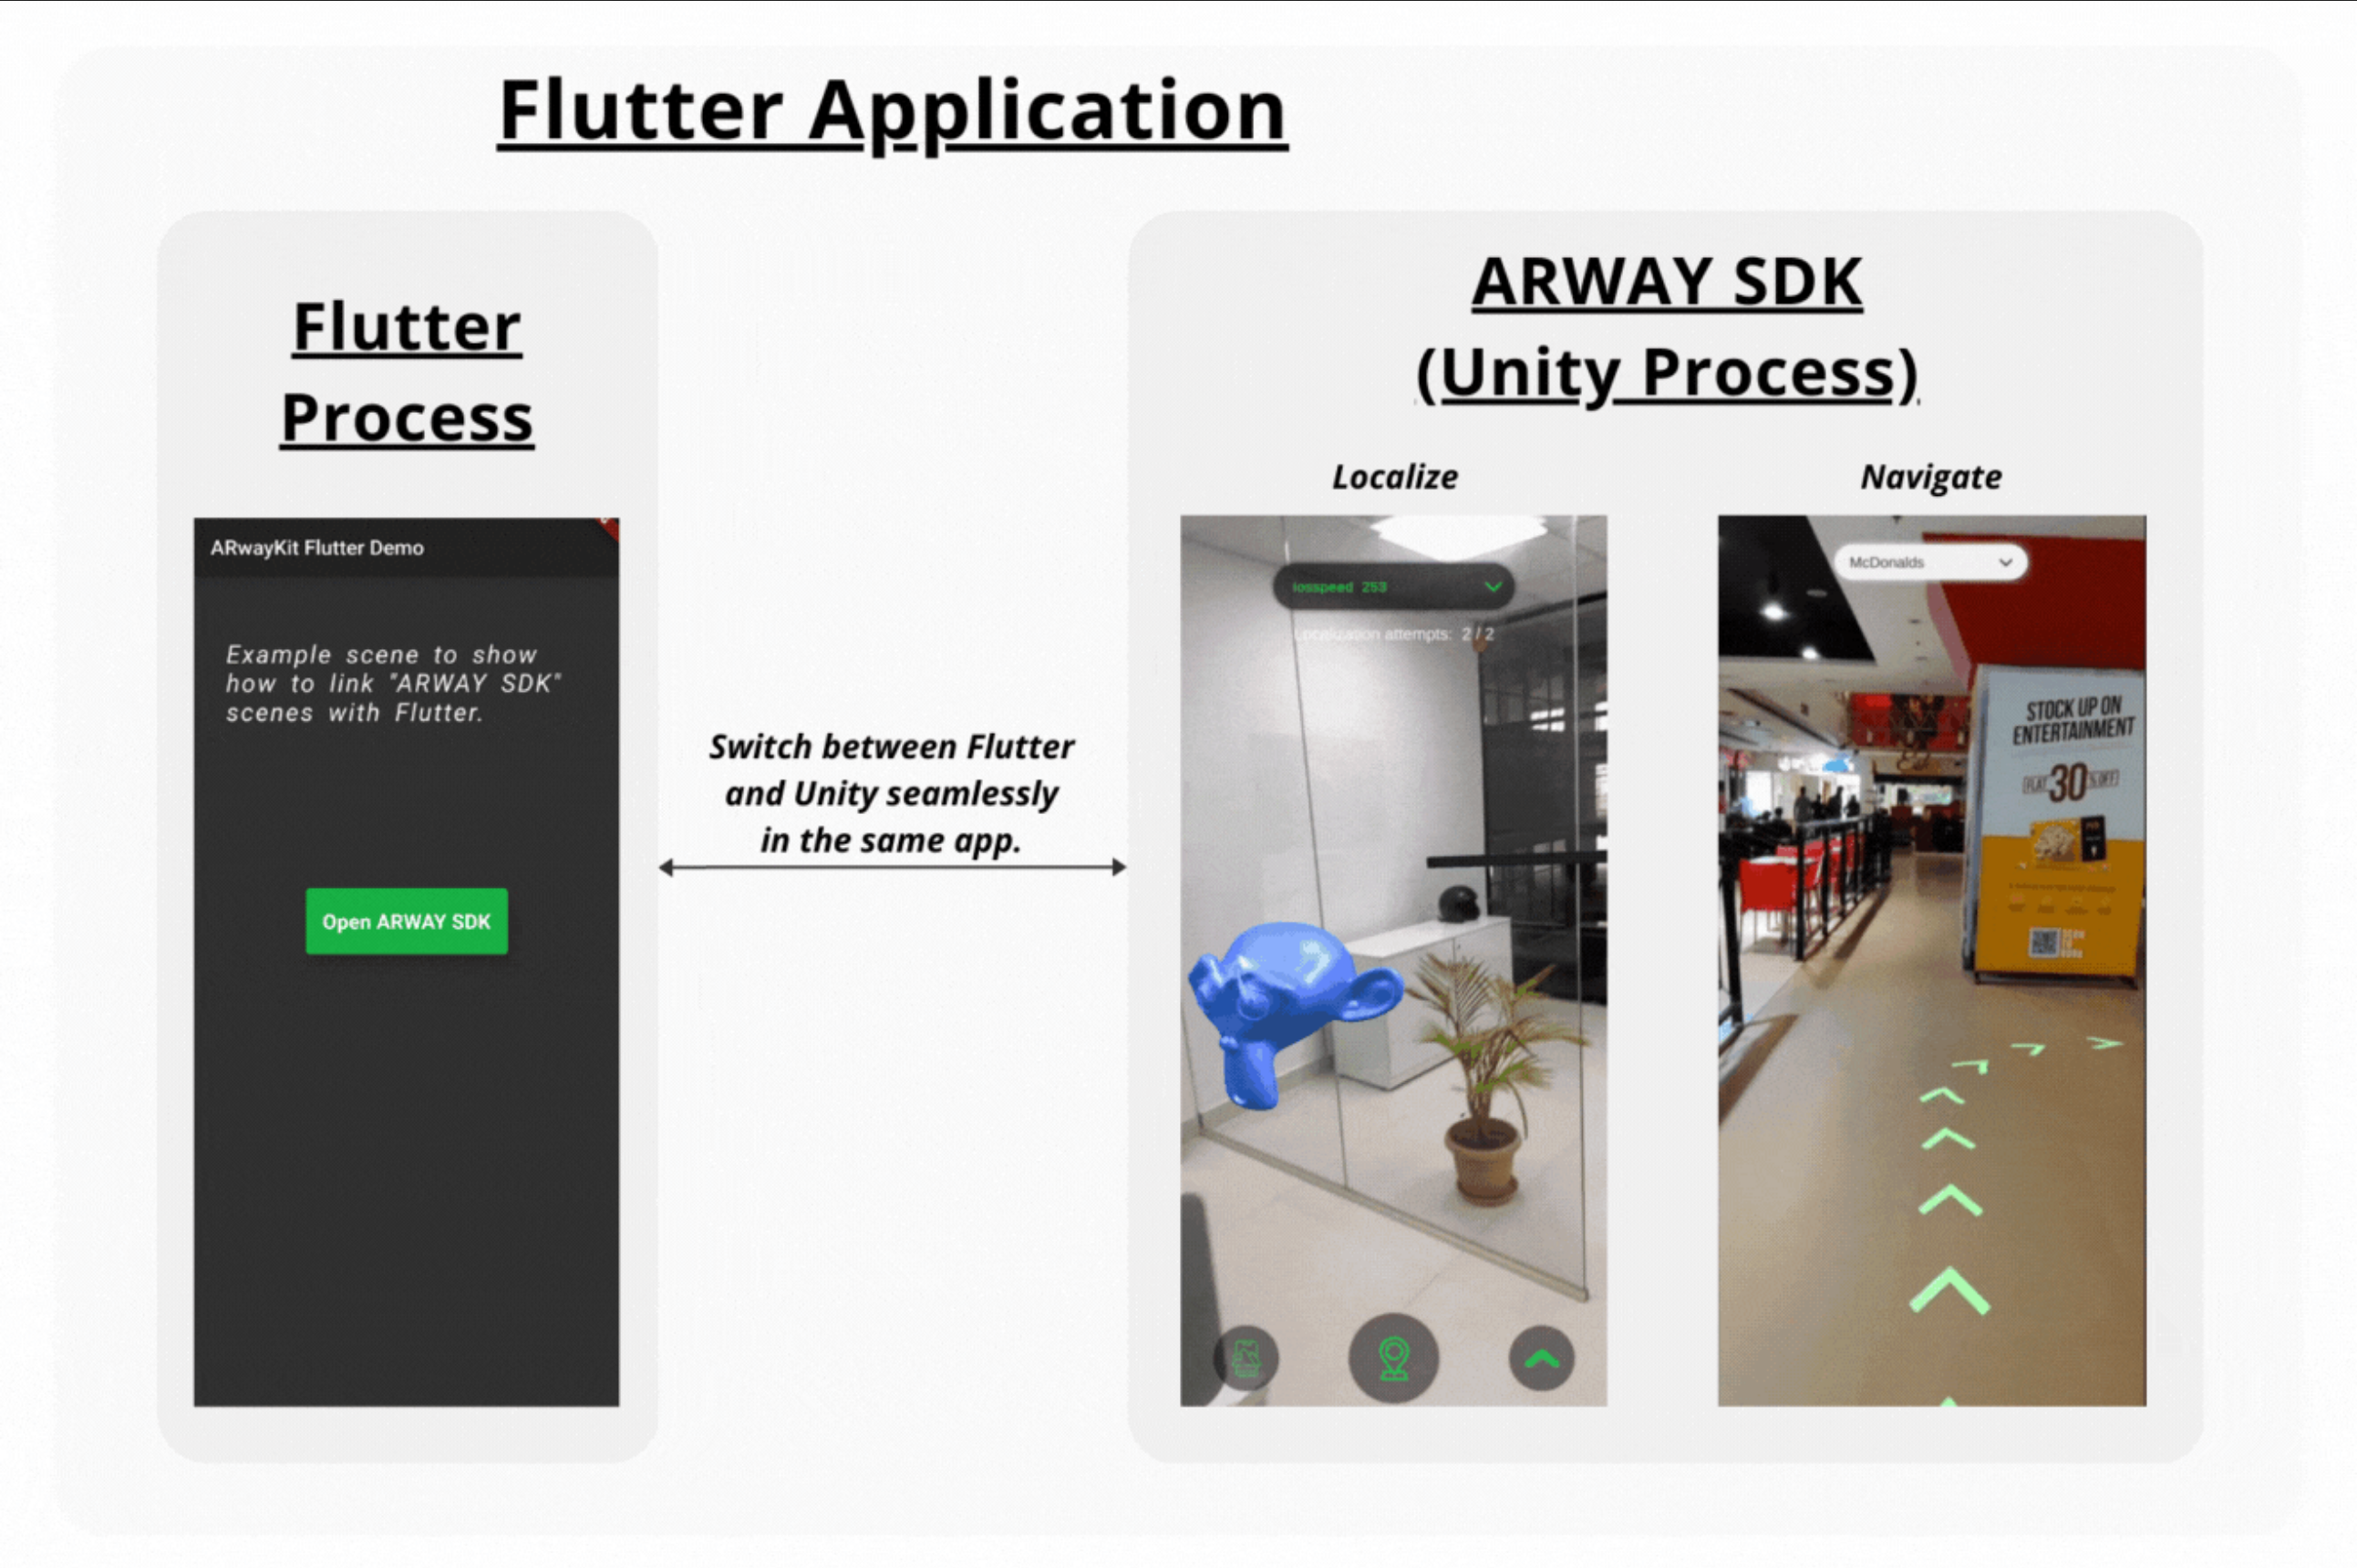
\includegraphics[width=\textwidth]{ARwayKit_samplegif_screenshot}
  \caption[Realtà aumentata con ARwayKit]{Immagine esempio di utilizzo realtà aumentata con ARwayKit\footnotemark}
\end{figure}
\footnotetext{Fonte: \url{https://medium.com/arway/building-ar-navigation-apps-with-flutter-and-arwaykit-280b69401cd9}}

Tuttavia, presenta delle criticità: in primo luogo obbliga l'uso di Unity (sfruttando la sua caratteristica peculiare di poter essere importato come fosse una libreria) per sviluppare la vista in realtà aumentata, il che comporta non solo dover imparare il linguaggio ma dover anche configurare ulteriori componenti (come ad esempio Unity Hub) che poi devono essere adottati assieme a quelli già in uso, appesantendo quindi il processo di codifica.\\
In secondo luogo troviamo invece il problema maggiore: la vista verrebbe realizzata nativamente in Unity, ovvero si tratta di una componente Unity separata rispetto all'applicazione che la lancia.
Questo renderebbe complesso se non impossibile usare dentro essa delle funzionalità Flutter: ad esempio, un bottone a schermo sarebbe un pulsante Unity, non Flutter, obbligando quindi poi a costruire una mappatura tra i due linguaggi per ogni funzionalità visualizzata.\\ 
Una vista così costruita non solo è scomoda da programmare, ma anche difficile da manutenere.

\subsubsection{ar\_flutter\_plugin}
\aplug{} è un \textit{plugin open-source} collaborativo estremamente giovane (il primo \textit{commit} sulla \textit{repository} pubblica risale al 6 febbraio 2021\footnote{Fonte: \url{https://github.com/CariusLars/ar_flutter_plugin/commit/da9ab148219d833755ef7a9b1e3536a3cae865d1}}) che si pone l'obiettivo di implementare componenti in realtà aumentata in Flutter.\\
Per raggiungere lo scopo si serve della libreria archiviata Sceneform\footnote{Fonte: \url{https://developers.google.com/sceneform/develop}}, che si occupa di "renderizzare scene tridimensionali realistiche in applicazioni in realtà aumentata o meno, senza dover imparare OpenGL".\\
L'architettura di \aplug{} è composta da due componenti: una \api{} multipiattaforma unificata che fornisce un'interfaccia alle applicazioni tramite il \textit{plugin} e le implementazioni specifiche per le piattaforme Android (in Kotlin) e iOS (in Swift) costruite su ARCore e ARKit rispettivamente, così da garantire accesso continuativo nel tempo a funzionalità aggiornate.\\
\aplug{} espone dei \textit{widget} che possono essere inclusi nel \textit{widget tree} (fig. \ref{fig:flutter-trees}) dell'applicazione cliente e delle classi \textit{manager} per gestire funzionalità e logiche di controllo del \textit{plugin} e delle componenti in realtà aumentata: il \textit{session manager} gestisce le configurazioni di tracciamento (ad esempio se gestire piani orizzontali, verticali o entrambi), opzioni di \textit{debugging} (come la visualizzazione dei piani) e le \textit{callbacks} per gli \textit{hit-test}\footnote{Immaginando un vettore che parte dall'ottica del dispositivo e tocca una superficie, possiamo considerare quel contatto un \textit{"hit"}. Con \textit{hit-testing} si intende valutare la capacità di tracciare correttamente lo spazio inteso come distanza tra i punti dello stesso e il dispositivo.} e i \textit{gesture events}\footnote{Azioni che il sistema deve fare quando vengono effettuati degli \textit{input} tramite \textit{touch screen} del dispositivo}.\\
L'\textit{object manager} gestisce i nodi in realtà aumentata del \textit{plugin} che servono ad astrarre rispetto alle funzionalità native delle varie piattaforme (ARCore e ARKit ad esempio) e permettono di aggiungere, modificare o rimuovere nodi basandosi su formati GLTF2 o GLB che possono essere caricati a \textit{runtime} da un \textit{file system} o dalla rete.\\
L'\textit{anchor manager} contiene funzioni per caricare e ottenere ancoraggi da servizi \textit{cloud} servendosi della \api{} Google Coud Anchor. Gli ambienti virtuali registrati localmente possono essere salvati in rete e comparati con quelli già in \textit{storage} persistente per scaricare ancoraggi e oggetti precedentemente posizionati nella scena.\\
Infine il \textit{location manager} si occupa di fornire le coordinate del \textit{global positioning system}  per permettere un'interrogazione efficiente degli ancoraggi basati su posizione geografica.\\
Il \textit{plugin} ha un'architettura largamente \textit{clout-agnostic}, ovvero che non si interessa dell'implementazione specifica per i servizi di salvataggio persistente, il che gli permette di usare facilmente gestori di contenuti esterni.

\subsubsection{Confronto}

\subsection{Analisi dei requisiti}
Di seguito sono riportati i requisti individuati nel piano di lavoro proposto e a seguito di opportuni confronti con il tutor aziendale. Essi sono catalogati secondo la dicitura:
\begin{center}
    \textbf{R[Obbligatorietà][Tipologia][Codice]}
\end{center}
dove:
\begin{itemize}
    \item \textbf{Obbligatorietà}: specifica quanto un requisito sia vincolante per la riuscita del prodotto e può assumere i seguenti valori:
    \begin{itemize}
        \item \textbf{1: } Requisito obbligatorio;
        \item \textbf{2: } Requisito desiderabile ma non essenziale per il funzionamento;
        \item \textbf{3: } Requisito opzionale.
    \end{itemize}
    \item \textbf{Tipologia}: specifica la tipologia del requisito e può assumere i seguenti valori:
    \begin{itemize}
        \item \textbf{F: }\textit{funzionale,} determina una funzionalità necessaria all'applicazione;
        \item \textbf{V: }\textit{vincolo,} riguarda una caratteristica del prodotto decisa a monte.
    \end{itemize}
    \item \textbf{Codice}: identifica univocamente un requisito all'interno della sua tipologia (ovvero possono esistere due requisiti con lo stesso codice a patto che siano uno funzionale e uno di vincolo). Per i requisti subordinati si usa il "punto" come divisorio (\textit{ReqPadre, ReqPadre.Figlio1})
\end{itemize}

\subsubsection{Requisiti funzionali}
{
    \setlength{\freewidth}{\dimexpr\textwidth-10\tabcolsep}
    \renewcommand{\arraystretch}{1.5}
    \centering
    \setlength{\aboverulesep}{0pt}
    \setlength{\belowrulesep}{0pt}
    \rowcolors{2}{red!10}{white}
    \begin{longtable}{C{.15\freewidth} | C{1\freewidth}}
       \toprule
    \rowcolor{red}
    \textcolor{white}{\textbf{Codice}}&
    \textcolor{white}{\textbf{Descrizione}}\\
    \toprule
    \endhead

    R1F1 & Il \textit{plugin} deve rappresentare \textit{asset} tramite ancoraggio in realtà aumentata\\
    R1F2 & Il \textit{plugin} deve rappresentare \textit{ticket} tramite ancoraggio in realtà aumentata\\
    R1F3 & Il \textit{plugin} deve integrare gli ancoraggi tramite \asa{}\\
    R1F3.1 & Permettere aggiunta di \asa\\%C
    R1F3.2 & Permettere recupero e visualizzazione di \asa\\%R
    R2F3.3 & Permettere modifica di \asa\\%U
    R1F3.4 & Permettere eliminazione di \asa\\%D
    %API BACKEND
    R1F4 & Comunicare con le \api{}s di Syn\\
    R1F4.1 & Ricevere \textit{asset} con ancoraggio associato\\
    R1F4.2 & Aggiungere \textit{asset} con ancoraggio associato\\
    R2F4.3 & Ricevere \textit{ticket} con ancoraggio associato\\
    R2F4.4 & Aggiungere \textit{ticket} con ancoraggio associato\\
    %UI FLUTTER
    R1F5 & Utente deve poter vedere quali \textit{asset} hanno ancoraggio associato\\
    R2F6 & Utente deve poter vedere quali \textit{ticket} hanno ancoraggio associato\\
    R1F7 & Utente deve poter raggiungere l'ancoraggio in vista in realtà aumentata dalla schermata dell'\textit{asset}\\
    R1F8 & \textit{On-Tap} su una ancoraggio deve aprire una \textit{bottom sheet} contestuale\\
    R1F8.1 & \textit{Bottom sheet} deve presentare identificatore per \textit{asset} o \textit{ticket} associato alla ancoraggio\\
    R1F8.2 & \textit{Bottom sheet} associato a un \textit{asset} mostra ultimi tre \textit{ticket} aperti\\
    R1F8.3 & \textit{Bottom sheet} deve fornire \textit{Call-To-Action} per eliminare l'ancoraggio\\
    R1F8.4 & \textit{Bottom sheet} deve fornire \textit{Call-To-Action} per raggiungere pagina di dettaglio\\
    R1F9 & Le informazioni contestuali di un \textit{ticket} includono data e ora di creazione\\
    %UI AR
    R1F10 & Gli ancoraggi hanno rappresentazione visiva contestuale\\ 
    R1F10.1 & Gli \textit{asset} vengono rappresentati come \todo\\
    R1F10.2 & I \textit{ticket} vengono rappresentati come \todo\\
    R1F11 & \textit{On-Tap} sullo spazio permette di creare una ancoraggio in posizione\\
    R1F11.1 & Ancoraggio posizionato nello spazio può essere salvato\\
    R1F11.2 & Ancoraggio posizionato nello spazio può essere eliminato\\
    R1F12 & Il salvataggio di un'ancoraggio è disponibile solo quando è sicuro vada a buon fine\\
    R1F12.1 & Viene mostrato a schermo un feedback riguardo il livello di sicurezza raggiunto\\
    \bottomrule
    \rowcolor{white} 
    \caption{Tabella dei requisiti funzionali}
    \label{tab:requisiti-funzionali}
    \end{longtable}
}

\subsubsection{Requisiti di vincolo}
{
    \setlength{\freewidth}{\dimexpr\textwidth-10\tabcolsep}
    \renewcommand{\arraystretch}{1.5}
    \centering
    \setlength{\aboverulesep}{0pt}
    \setlength{\belowrulesep}{0pt}
    \rowcolors{2}{red!10}{white}
    \begin{longtable}{C{.15\freewidth} C{1\freewidth}} 
       \toprule
    \rowcolor{red}
    \textcolor{white}{\textbf{Codice}}&
    \textcolor{white}{\textbf{Descrizione}}\\
    \toprule
    \endhead

    R1V1 & \textit{Framework} scelto funziona su Android\\
    R2V2 & \textit{Framework} scelto funziona su iOS\\
    R1V3 & \textit{Framework} scelto si integra con le \api{}s di Syn\\
    R1V3.1 & \textit{Framework} ottiene con ancoraggio associato i dati degli \textit{asset}\\
    R1V3.2 & \textit{Framework} ottiene con ancoraggio associato i dati dei \textit{ticket}\\
    R1V4 & Il \textit{framework} scelto utilizza asa\\
    R1V5 & La vista in realtà aumentata deve essere sviluppata in Flutter\\
    \bottomrule
    \rowcolor{white} 
    \caption{Tabella dei requisiti di vincolo}
    \label{tab:requisiti-di-vincolo}
    \end{longtable}
}

\subsubsection{Riepilogo requisiti}
Sono stati individuati un totale di 36 requisiti, 29 funzionali e 7 di vincolo, di seguito schematizzati:
{
    \setlength{\freewidth}{\dimexpr\textwidth-10\tabcolsep}
    \renewcommand{\arraystretch}{1.5}
    \centering
    \setlength{\aboverulesep}{0pt}
    \setlength{\belowrulesep}{0pt}
    \rowcolors{2}{red!10}{white}
    \begin{longtable}{C{.25\freewidth} C{.2\freewidth}} 
       \toprule
    \rowcolor{red}
    \textcolor{white}{\textbf{Obbligatorietà}}&
    \textcolor{white}{\textbf{Quantità}}\\
    \toprule
    \endhead

    Obbligatori & 31\\
    Desiderabili & 5\\
    \bottomrule
    \rowcolor{white} 
    \caption{Numero di requisiti per obbligatorietà}
    \label{tab:requisiti-obbligatorieta}
    \end{longtable}
}

{
    \setlength{\freewidth}{\dimexpr\textwidth-10\tabcolsep}
    \renewcommand{\arraystretch}{1.5}
    \centering
    \setlength{\aboverulesep}{0pt}
    \setlength{\belowrulesep}{0pt}
    \rowcolors{2}{red!10}{white}
    \begin{longtable}{C{.25\freewidth} C{.2\freewidth}} 
       \toprule
    \rowcolor{red}
    \textcolor{white}{\textbf{Tipologia}}&
    \textcolor{white}{\textbf{Quantità}}\\
    \toprule
    \endhead

    Funzionali & 29\\
    Di Vincolo & 7\\
    \bottomrule
    \rowcolor{white} 
    \caption{Numero di requisiti per tipologia}
    \label{tab:requisiti-tipolgia}
    \end{longtable}
}

\subsection{Attività di supporto}
\subsubsection{Interazione aziendale}
\subsubsection{Processi di verifica e validazione}
%************************************************************************************************************
\section{Difficoltà incontrate}
\subsection{Problemi documentali}
\subsection{Problemi tecnologici}

%************************************************************************************************************

\section{Risultati raggiunti}
\subsection{Copertura requisiti}
\subsection{Implementazione Android}
\subsection{Implementazione iOS}

% !TEX encoding = UTF-8
% !TEX TS-program = pdflatex
% !TEX root = ../tesi.tex

%**************************************************************
\chapter{Valutazione Retrospettiva}
\label{cap:valutazione-retrospettiva}
%**************************************************************

\section{Soddisfacimento obiettivi}
\subsection{Valutazione personale}
\subsection{Valutazione proponente}

\section{Competenze}
\subsection{Competenze acquisite}
\subsection{Competenze mancanti}
\subsubsection{Lacune corso di studi}


\iffalse
% !TEX encoding = UTF-8
% !TEX TS-program = pdflatex
% !TEX root = ../tesi.tex

%**************************************************************
\chapter{Introduzione}
\label{cap:introduzione}
%**************************************************************

\section{L'azienda}
\begin{figure}[ht]
    \centering
    \includegraphics[height=3cm]{ds_logo}
    \caption{Logo Datasoil S.r.l.}
\end{figure} 
\aCapo{}
Datasoil S.r.l. è una startup innovativa che si occupa di sviluppare applicativi dedicati alla gestione aziendale, altamente integrati con industria 4.0 e Digital Twin: vengono impiegati machine learning e analisi predittive per ottenere analitiche migliori rispetto alla concorrenza, con un occhio attento a innovazione, sicurezza e scalabilità, ottenute tramite prototipazione, MVP e Infrastrucutre as Code, delegando quindi la gestione delle componenti Server a servizi terzi come AWS.\\
Il loro obiettivo è manipolare ed elaborare dati di natura inerentemente caotica, ordinarli e presentarli all'utente finale con UI intuitive e interattive, promuovendo un'interazione efficace tra utilizzatore e mezzo. Prediligono un approccio ai problemi condiviso e modulare per far nascere soluzioni inedite da applicare a grandi progetti, forti di un know-how che abbraccia esigenze verticali.\\
Le piattaforme dedicate ad industry 4.0, smart building e smart city poggiano su dei data silos attualmente esistenti, garantendo un'interpretazione integrata e di alto livello delle informazioni aziendali fondendole con eventi provenienti dai diversi business level creando insight proattivi in tempo reale. I sistemi predittivi di Datasoil sono in grado di notificare la persona giusta al momento giusto anticipando la gestione delle criticità interfunzionali.

%**************************************************************
\section{Il progetto e lo stage}

\subsection{Descrizione}
Il progetto proposto prevede l'implementazione di una vista in realtà aumentata per l'applicazione di ticketing e monitoraggio aziendale "\textbf{SYN}".\\
La componente AR dovrà necessariamente appoggiarsi al servizio di \gls{asa} perchè gli \gls{asset} aziendali tracciati da \textbf{SYN} hanno un \gls{digital twin} ancorato e localizzato proprio tramite le \gls{anchor} di Microsoft, e dovrà idealmente essere cross-platform quindi fornendo l'implementazione adeguata sia per Android che per iOS.\\
Dalla vista dovrà essere possibile interagire con gli \gls{asset}, quindi ottenendoli dal cloud e presentandoli nella scena AR, e con i ticket a loro associati, provocando l'apparizione di una card all' on-tap dell'\gls{asset}, ovvero mostrando a schermo tramite una lista testuale i vari ticket relativi all'\gls{asset} dopo che questo viene toccato.\\
Per concludere l'interezza degli obiettivi sarà necessario studiare dei \gls{framework} o degli \gls{SDK} che permettono l'integrazione di \gls{asa} in codice nativo (che sarà Java per Android e Swift per iOS) con il \gls{framework} Flutter e il linguaggio su cui si poggia, ovvero Dart.


\subsection{Obiettivi}
\begin{itemize}
    \item Minimi:
        \begin{itemize}
            \item Studio e comprensione del linguaggio di programmazione \textit    {Dart} e del \gls{framework} \textit{Flutter};
            \item Analisi toolkit Azure: Azure Console e \gls{asa};
            \item Ricerca di \gls{framework} e \gls{SDK} per implementare le \gls   {asa} in \textit{Flutter};
            \item Eventuale studio di linguaggi ulteriori necessari alle    implementazioni native, come ad esempio \textit{Kotlin}, \textit{Java},    \textit{Unity} o \textit{Swift};
            \item Completamento del \gls{framework} scelto nell'app \textit{Flutter}    esistente;
            \item Completamento dello sviluppo dei componenti per rappresentare le \Gls{anchor} nello spazio AR;
            \item Completamento dello sviluppo delle \acrshort{api} per l'interazione utente con le \Gls{anchor} AR;
        \end{itemize}
    \item Massimi: 
        \begin{itemize}
            \item Sviluppo di componenti per mappare \gls{asset} aziendali ad \Gls{anchor} AR;
            \item Sviluppo di componenti UI per la visualizzazione di metriche e informazioni di controllo.
        \end{itemize}
\end{itemize}



\subsection{Pianificazione del lavoro}
\todo probabile necessità di modifica, ora è più rendicontazione.
\begin{itemize}
    \item \textbf{Settimana 1:} 
        \begin{itemize}
            \item Installazione e configurazione del framework \flutter, della SDK Android 
            \item Configurazione emulatore Android (scelto Pixel 6 API 33) e 
            developers options sul mio telefono personale;
            \item Configurazione \vsc e \astudio;
            \item Sviluppo di piccola app d'esempio con \flutter che sfrutta gli \textit{Stateful Widgets};
        \end{itemize} 
    \item \textbf{Settimana 2:} 
        \begin{itemize}
            \item Studio degli \textit{Hook Widgets}, simili agli \textit{Hooks} di \textit{Rest};
            \item Traduzione degli \textit{Stateful Widgets} dell'app d'esempio in \textit{Hook Widgets};
            \item Sviluppo app d'esempio con gli \textit{Hook Widgets};
        \end{itemize}
    \item \textbf{Settimana 3:} 
        \begin{itemize}
            \item Studio delle asa;
            \item Creazione risorse necessarie nel portale di \textit{Azure};
            \item Deploy app di esempio fornita da \textit{Microsoft};
        \end{itemize}
    \item \textbf{Settimana 4:} Studio dei metodi per implementare le asa in \flutter:
        \begin{itemize}
            \item Studio dei \textit{Method Channels};
            \item Studio di \textit{ARwayKit} e valutazione del suo approccio tramite \unity;
            \item Studio di \arplug;
        \end{itemize}
    \item \textbf{Settimana 5:} 
        \begin{itemize}
            \item Adattamento dell'esempio \arplug per integrarci le asa;
            \item Lettura dei logs per filtrarne gli output;
        \end{itemize}
    \item \textbf{Settimana 6:} Utilizzo diretto di \arcore in \flutter per capirne il workflow;
    \item \textbf{Settimana 7:} Integrazione di asa in \flutter senza errori;
    \item \textbf{Settimana 8:} Integrazione di componenti AR in SYN;
\end{itemize}
%************************************************************************************************************
\section{Prodotto ottenuto}
\todo

\iffalse
Il prodotto ottenuto si compone di due diverse applicazioni: applicazione cliente e applicazione coach.\\
Entrambe le applicazioni sono state sviluppate utilizzando \textit{Flutter} come framework in modo da valutarne anche le potenzialità, infatti l'azienda ha sempre utilizzato React Native per lo sviluppo mobile. Mentre per lo stile dei componenti dell'applicazione si è deciso di utilizzare il \textit{Material Design} di Google già ampiamente utilizzato da Datasoil S.r.l.\\
L'applicazione cliente allo stato attuale permette la visione dei propri obiettivi di movimento e degli appuntamenti, oltre che una schermata di profilo personale con la possibilità di associazione ai diversi profili fitness al fine di rilevare dati.\\
L'app cliente è quindi a circa un terzo dello sviluppo, l'azienda ora potrà continuare con lo sviluppo delle restanti sezioni relative alla dieta e alla visualizzazione dello stato di salute del cliente. \\
L'applicazione coach allo stato attuale permette la visualizzazione della lista dei propri clienti con i relativi obiettivi di movimento e la visualizzazione di un'agenda con gli appuntamenti. L'app coach è in buona parte sviluppata, l'idea aziendale è quella che dall'app il coach possa solo vedere ciò che ha già assegnato dall'interfaccia web (prodotto già sviluppato da Datasoil S.r.l.). \\
L'azienda quindi dovrà solo aggiungere la visualizzazione della dieta e dei parametri di salute del cliente, omettendo la possibilità di assegnare ulteriori obiettivi dall'app mobile. 
Per entrambe le applicazioni è stata predisposta una versione minimale di chat in modo che il cliente possa comunicare con il proprio coach. Questa chat sarà in futuro ampiamente rivista in modo da permettere lo scambio di file multimediali e di video chiamate, oltre che limitare lo scambio di messaggi tramite una sorta di abbonamento.
\fi
%************************************************************************************************************
\section{Difficoltà incontrate}
Le difficoltà primariamente incontrate sono state tre: comprensione dei mezzi da usare, farli comunicare tra loro e la scarsissima assistenza trovata online.\\
Infatti la necessità di familiarizzare in poco tempo con molte componenti (linguaggi, framework, plug-in, SDKs) diverse e mai viste prima, come \flutter, \kotlin, \java, \dart, Android SDK, asa, \arcore e \arplug si è certamente dimostrato complesso, tuttavia non quanto lo è stato far comunicare queste componenti delle quali non ho esperienza tra di loro: ad esempio implementando in \flutter (quindi \dart), sfruttando l'\arplug (che usa \kotlin e \flutter), le asa (scritte in \java) che a loro volta si appoggiano ad \arcore (così come lo fa, in una certa parte, \arplug). \\
Tutto questo è stato esacerbato dalla scarsissima documentazione fornita da \textit{Microsoft} per le asa e dalle pochissime risorse online (compresi forum e issue di \textit{GitHub}) riguardo all'implementazione AR in generale, \textit{ASA} nello specifico, in \flutter.
%**************************************************************
\section{Struttura della relazione}

\begin{description}
    \item[{\hyperref[cap:strumenti-utilizzati]{Il secondo capitolo}}] descrive gli strumenti e le tecnologie utilizzate per svolgere il progetto, particolare attenzione è posta sulla presentazione del framework Flutter, in quanto è alla base del prodotto ottenuto;
    
    \item[{\hyperref[cap:analisi-requisiti]{Il terzo capitolo}}] espone un'analisi tecnica dei requisiti individuati che il prodotto finale deve soddisfare al termine del periodo di stage;
    
    \item[{\hyperref[cap:progettazione]{Il quarto capitolo}}] descrive le scelte progettuali adottate per ottenere una struttura solida manutenibile;
    
    \item[{\hyperref[cap:sviluppo]{Il quinto capitolo}}] espone il percorso di realizzazione del prodotto e le soluzioni alle difficoltà incontrate;
    
    \item[{\hyperref[cap:conclusioni]{Il sesto capitolo}}] descrive l'esperienza di stage e i risultati ottenuti.
\end{description}

Riguardo la stesura del testo, relativamente al documento sono state adottate le seguenti convenzioni tipografiche:
\begin{itemize}
	\item gli acronimi, le abbreviazioni e i termini ambigui o di uso non comune menzionati vengono definiti nel glossario, situato alla fine del presente documento;
	\item i termini in lingua straniera o facenti parti del gergo tecnico sono evidenziati con il carattere \emph{corsivo}.
\end{itemize}
             % Introduzione
% !TEX encoding = UTF-8
% !TEX TS-program = pdflatex
% !TEX root = ../tesi.tex

%**************************************************************
\chapter{Strumenti utilizzati}
\label{cap:strumenti-utilizzati}
%**************************************************************

\section{Strumenti di sviluppo}
\subsection{Visual Studio Code}
\begin{figure}[ht]
    \centering
    \includegraphics[height=2cm]{vsc_logo}
    \caption{Logo di Visual Studio Code}
\end{figure} \aCapo{}
\vsc{} è un editor per codice sorgente, sviluppato da \textit{Microsoft} servendosi del framework \textit{Electron}, disponibile per Windows, Linux e macOS. Le sue funzionalità comprendo supporto per debugging, syntax highlighting, intelligent code completion, snippets, code refactoring, e integrazione con Git. \\
Gli utenti possono configurare tema, macro, preferenze e installare estensioni che ne aumentano le funzionalità aggiungendo ad esempio il supporto ai maggiori linguaggi di porgrammazione attualmente presenti.\\
Nella \textit{Stack Overflow 2021 Developer Survey}, \vsc{} è risultato essere l'IDE più popolare, adottato dal 70\% degli intervistati. {\tiny Fonte: \href{https://en.wikipedia.org/wiki/Visual_Studio_Code}{Wikipedia}}\\
\E{} inoltre presente e molto comoda l'estensione di \flutter{} che, tra le altre cose, permette di gestire direttamente in gui i vari dispositivi (smartphone, browser o emulatore) sui quali installare e lanciare l'app che si sta programmando.

\subsection{Android Studio}
\begin{figure}[ht]
    \centering
    \includegraphics[height=2cm]{as_logo}
    \caption{Logo di Android Studio}
\end{figure}\aCapo{}
\textit{Android Studio} è l'IDE ufficiale del sistema operativo di Gooogle, sostituendo Eclipse dal 2015, costruito sul software IntelliJ di JetBrains e progettato specificatamente per lo sviluppo Android. \E{} disponibile per Windows, Linux e macOS.\\
Il 7 maggio 2019 Kotlin rimpiazzò Java come linguaggio consigliato per Android, favorendo un'integrazione ancora maggiore con JetBrains che, appunto, ha sviluppato e prodotto Kotlin stesso. {\tiny Fonte: \href{https://en.wikipedia.org/wiki/Android_Studio}{Wikipedia}}\\
Personalmente ho cercato nonostante tutto di programmare il più possibile su \vsc{} preferendolo quindi ad \textit{Android Studio} in virtù della sua maggiore leggerezza e delle sue più ampie possibilità di personalizzazione.

\subsection{Dart}
\begin{figure}[ht]
    \centering
    \includegraphics[height=2cm]{dart_logo}
    \caption{Logo di Dart}
\end{figure} \aCapo{}
Dart è un linguaggio di programmazione sviluppato da Google per il client development, ovvero per web e mobile app, e può anche essere impiegato per la costruzione di applicazione desktop e server.\\
\E{} un linguaggio object-oriented, class-based, garbage-collected, strongly-typed e con una sintassi nello stile di C. Può compilare sia codice macchina che JavaScript e supporta interefacce, mixins, classi astratte, refined generics e type inference.{\tiny Fonte: \href{https://en.wikipedia.org/wiki/Dart_(programming_language)}{Wikipedia}}\\
Personalmente l'ho trovato elegante e conciso nella sua struttura, e presenta dei vantaggi consistenti come la null protection e le espressioni ternarie.

\subsection{Flutter}
\begin{figure}[ht]
    \centering
    \includegraphics[height=2cm]{flutter_logo}
    \caption{Logo di Flutter}
\end{figure} \aCapo{}
Flutter è un framework open-source creato da Goole per lo sviluppo della UI di applicazioni cross-platform per Android, iOS, Linux, macOS, Windows, Google Fuchsia e il web partendo da un singolo codebase.\\
Rialsciato a maggio 2017, le applicazioni in Flutter sono scritte in Dart e sfruttano molte delle features avanzate del linguaggio, e le componenti principali del framework sono:
\begin{itemize}
    \item \textbf{Dart platform:} Flutter gira all'interno della Dart Virtual Machine, che si serve di un execution engine just-in-time;
    \item \textbf{Flutter engine:} scritto primariamente in C++, fornisce supporto a basso livello per il rendering e implementa accessibilità, file e network I/O, supporto nativo per i plugin e molto altro;
    \item \textbf{Foundation library:} scritta in Dart, fornisce classi e funzioni di base che vengono usate per costruire gli applcativi in Flutter, come ad esempio le API per la comunicazione con l'engine;
    \item \textbf{Design-specific widgets:} Flutter contiene due famiglie di widget che si conformano a delle specifiche scuole di design: \textit{Material} per Google e \textit{Cupertino} per Apple;
    \item \textbf{Flutter DevTools:} famiglia di tools generici che vengono sfruttati per lo sviluppo di software in Flutter.
\end{itemize}
~\\
Inoltre, una libreria fondamentale per semplificare l'utilizzo di Flutter è \textit{Flutter Hooks}: lo scopo è implementare delle strutture simili agli Hooks di React, consentono di sostituire gli Stateful Widget riducendo il boilerplate code e semplificando la gestione di side-effect e ciclo di vita dei widget grazie alla funzione \textit{useEffect}.

\subsection{Java}
\begin{figure}[ht]
    \centering
    \includegraphics[height=4cm]{java_logo.png}
    \caption{Logo di Flutter}
\end{figure} \aCapo{}

\subsection{Kotlin}
\begin{figure}[ht]
    \centering
    \includegraphics[height=1.5cm]{kotlin_logo.png}
    \caption{Logo di Flutter}
\end{figure} \aCapo{}

\subsection{Azure Spatial Anchors}
\begin{figure}[ht]
    \centering
    \includegraphics[height=2.5cm]{asa_logo.png}
    \caption{Logo di Flutter}
\end{figure} \aCapo{}

\subsection{ARCore}
\begin{figure}[ht]
    \centering
    \includegraphics[height=2cm]{arcore_logo.png}
    \caption{Logo di Flutter}
\end{figure} \aCapo{}
%**************************************************************
\section{Strumenti organizzativi}

\subsection{Slack}
\begin{figure}[ht]
    \centering
    \includegraphics[height=1.5cm]{slack_logo}
    \caption{Logo di Slack}
\end{figure}

Slack è un software che rientra nella categoria degli strumenti di collaborazione aziendale utilizzato per inviare messaggi in modo istantaneo ai diversi membri del team.\\
Slack è utilizzabile da browser, applicazione desktop e applicazione o mobile.\\
Oltre ai messaggi diretti tra i membri è anche possibile creare diversi canali in modo da separare le conversazioni per argomento, per esempio nel nostro caso utilizzavamo due canali: \#frontend, \#backend.\\
Slack inoltre permette di integrare nel sistema di messaggistica anche altri servizi, come per esempio Github o Jira.

\subsection{Jira}
\begin{figure}[ht]
    \centering
    \includegraphics[height=3cm]{jira_logo.png}
    \caption{Logo di Jira}
\end{figure}

Jira è un software utilizzato per gestire il lavoro collaborativo, segue il principio agile e permette di creare ticket e gestire degli sprint settimanali.\\ Nel nostro caso chiunque poteva aprire un ticket nella sezione \textit{TODO} e assegnarlo a chi di dovere, specificandone i dettagli. Quando il ticket veniva preso in carico lo si spostava nell' apposita sezione \textit{IN PROGRESS} e una volta terminato veniva chiuso nella sezione \textit{DONE}. In questo modo ognuno sa in quale stato è il prodotto e a cosa sta lavorando ogni membro del team.


\subsection{Github}
\begin{figure}[ht]
    \centering
    \includegraphics[height=3cm]{github_logo}
    \caption{Logo di GitHub}
\end{figure}

GitHub è un servizio di hosting per progetti software ed è una implementazione del sistema di versionamento distribuito Git.\\ Il sito è principalmente utilizzato dagli sviluppatori, che caricano il codice sorgente dei loro programmi e lo possono rendere disponibile al resto degli utenti. Questi ultimi possono interagire con lo sviluppatore tramite un sistema di \textit{issue tracking}, \textit{pull request} e commenti che permette di migliorare il codice del \textit{repository} risolvendo bug o aggiungendo funzionalità.
             % Processi
% !TEX encoding = UTF-8
% !TEX TS-program = pdflatex
% !TEX root = ../tesi.tex

%**************************************************************
\chapter{Analisi dei requisiti}
\label{cap:analisi-requisiti}
%**************************************************************

\section{Requisiti individuati}

Di seguito sono riportati i requisti individuati nel piano di lavoro proposto e a seguito di opportuni confronti con il tutor aziendale. Essi sono catalogati secondo la dicitura:
\begin{center}
    \textbf{R[Obbligatorietà][Tipologia][Codice]}
\end{center}
dove:
\begin{itemize}
    \item \textbf{Obbligatorietà}: specifica quanto un requisito sia vincolante per la riuscita del prodotto e può assumere i seguenti valori:
    \begin{itemize}
        \item \textbf{1: } Requisito obbligatorio;
        \item \textbf{2: } Requisito desiderabile ma non essenziale per il funzionamento;
        \item \textbf{3: } Requisito opzionale.
    \end{itemize}
    \item \textbf{Tipologia}: specifica la tipologia del requisito e può assumere i seguenti valori:
    \begin{itemize}
        \item \textbf{F: }\textit{funzionale,} determina una funzionalità necessaria all'applicazione;
        \item \textbf{V: }\textit{vincolo,} riguarda una caratteristica del prodotto decisa a monte.
    \end{itemize}
    \item \textbf{Codice}: identifica univocamente un requisito all'interno della sua tipologia (ovvero possono esistere due requisiti con lo stesso codice a patto che siano uno funzionale e uno di vincolo). Per i requisti subordinati si usa il "punto" come divisorio (\textit{ReqPadre, ReqPadre.Figlio1})
\end{itemize}

\subsection{Requisiti funzionali}

{
    \setlength{\freewidth}{\dimexpr\textwidth-10\tabcolsep}
    \renewcommand{\arraystretch}{1.5}
    \centering
    \setlength{\aboverulesep}{0pt}
    \setlength{\belowrulesep}{0pt}
    \rowcolors{2}{red!10}{white}
    \begin{longtable}{C{.15\freewidth} | C{1\freewidth}}
       \toprule
    \rowcolor{red}
    \textcolor{white}{\textbf{Codice}}&
    \textcolor{white}{\textbf{Descrizione}}\\
    \toprule
    \endhead
    
\iffalse
    %INTEGRAZIONE FRAMEWORK SCELTO NELL'APP FLUTTER ESISTENTE
    &\\
    %SVILUPPO COMPONENTI PER RAPPRESENTARE ANCHOR IN AR
    &\\
    %SVILUPPO API PER INTERAZIONE UTENTE CON ANCHOR AR
    &\\
    %SVILUPPO COMPONENTI PER MAPPARE ASSET AZIENDALI AD ANCHOR AR
    &\\
    %SVILUPPO COMPONENTI UI PER VISUALIZZARE METRICHE ED INFO DI CONTROLLO
    &\\
\fi
    %AR
    R1F1 & Il plugin-in deve rappresentare asset tramite Anchor AR\\
    R1F2 & Il plugin-in deve rappresentare ticket tramite Anchor AR\\
    R1F3 & Il plug-in deve integrare le Anchor tramite asa\\
    R1F3.1 & Permettere aggiunta di asa\\%C
    R1F3.2 & Permettere recupero e visualizzazione di asa\\%R
    R2F3.3 & Permettere modifica di asa\\%U
    R1F3.4 & Permettere eliminazione di asa\\%D
    %API BACKEND
    R1F4 & Comunicare con Syn API\\
    R1F4.1 & Ricevere asset con Anchor associata\\
    R1F4.2 & Aggiungere asset con Anchor associata\\
    R2F4.3 & Ricevere ticket con Anchor associata\\
    R2F4.4 & Aggiungere ticket con Anchor associata\\
    %UI FLUTTER
    R1F5 & Utente deve poter vedere quali asset hanno anchor associata\\
    R2F6 & Utente deve poter vedere quali ticket hanno anchor associata\\
    R1F7 & Utente deve poter raggiungere l'anchor in vista AR dalla schermata dell'asset\\
    R1F8 & On-Tap su una anchor deve aprire una bottom sheet contestuale\\
    R1F8.1 & Bottom sheet deve presentare identificatore per asset o ticket associato alla anchor\\
    R1F8.2 & Bottom sheet associato a un asset mostra ultimi tre ticket aperti\\
    R1F8.3 & Bottom sheet deve fornire Call-To-Action per eliminare l'anchor\\
    R1F8.4 & Bottom sheet deve fornire Call-To-Action per raggiungere pagina di dettaglio\\
    R1F9 & Le informazioni contestuali di un ticket includono data e ora di creazione\\
    %UI AR
    R1F10 & Anchor hanno rappresentazione visiva contestuale\\ 
    R1F10.1 & Asset vengono rappresentati come \todo\\
    R1F10.2 & Ticket vengono rappresentati come \todo\\
    R1F11 & On-Tap sullo spazio permette di creare una Anchor in posizione\\
    R1F11.1 & Anchor posizionata nello spazio può essere salvata\\
    R1F11.2 & Anchor posizionata nello spazio può essere eliminata\\
    R1F12 & Il salvataggio di un'Anchor è disponibile solo quando è sicuro vada a buon fine\\
    R1F12.1 & Viene mostrato a schermo un feedback riguardo il livello di sicurezza raggiunto\\
    \bottomrule
    \rowcolor{white} 
    \caption{Tabella dei requisiti funzionali}
    \label{tab:requisiti-funzionali}
    \end{longtable}
}



\subsection{Requisiti di vincolo}

{
    \setlength{\freewidth}{\dimexpr\textwidth-10\tabcolsep}
    \renewcommand{\arraystretch}{1.5}
    \centering
    \setlength{\aboverulesep}{0pt}
    \setlength{\belowrulesep}{0pt}
    \rowcolors{2}{red!10}{white}
    \begin{longtable}{C{.15\freewidth} C{1\freewidth}} 
       \toprule
    \rowcolor{red}
    \textcolor{white}{\textbf{Codice}}&
    \textcolor{white}{\textbf{Descrizione}}\\
    \toprule
    \endhead

    R1V1 & Framework scelto funziona su Android\\
    R2V2 & Framework scelto funziona su iOS\\
    R1V3 & Framework scelto si integra con API Syn\\
    R1V3.1 & Framework ottiene con Anchor associata i dati degli asset\\
    R1V3.2 & Framework ottiene con Anchor associata i dati dei ticket\\
    R1V4 & Il framework scelto utilizza asa\\
    R1V5 & La vista AR deve essere sviluppata in Flutter\\
    \bottomrule
    \rowcolor{white} 
    \caption{Tabella dei requisiti di vincolo}
    \label{tab:requisiti-di-vincolo}
    \end{longtable}
}



\section{Riepilogo requisiti}
\subsection{Riepilogo requisiti app cliente}
Sono stati individuati un totale di 36 requisiti, 29 funzionali e 7 di vincolo, di seguito schematizzati:

{
    \setlength{\freewidth}{\dimexpr\textwidth-10\tabcolsep}
    \renewcommand{\arraystretch}{1.5}
    \centering
    \setlength{\aboverulesep}{0pt}
    \setlength{\belowrulesep}{0pt}
    \rowcolors{2}{red!10}{white}
    \begin{longtable}{C{.25\freewidth} C{.2\freewidth}} 
       \toprule
    \rowcolor{red}
    \textcolor{white}{\textbf{Obbligatorietà}}&
    \textcolor{white}{\textbf{Quantità}}\\
    \toprule
    \endhead

    Obbligatori & 31\\
    Desiderabili & 5\\
    \bottomrule
    \rowcolor{white} 
    \caption{Numero di requisiti per obbligatorietà}
    \label{tab:requisiti-obbligatorieta}
    \end{longtable}
}

{
    \setlength{\freewidth}{\dimexpr\textwidth-10\tabcolsep}
    \renewcommand{\arraystretch}{1.5}
    \centering
    \setlength{\aboverulesep}{0pt}
    \setlength{\belowrulesep}{0pt}
    \rowcolors{2}{red!10}{white}
    \begin{longtable}{C{.25\freewidth} C{.2\freewidth}} 
       \toprule
    \rowcolor{red}
    \textcolor{white}{\textbf{Tipologia}}&
    \textcolor{white}{\textbf{Quantità}}\\
    \toprule
    \endhead

    Funzionali & 29\\
    Di Vincolo & 7\\
    \bottomrule
    \rowcolor{white} 
    \caption{Numero di requisiti per tipologia}
    \label{tab:requisiti-tipolgia}
    \end{longtable}
}
             % Kick-Off
% !TEX encoding = UTF-8
% !TEX TS-program = pdflatex
% !TEX root = ../tesi.tex

%**************************************************************
\chapter{Progettazione}
\label{cap:progettazione}
%**************************************************************
\section{Organizzazione repository e sistema di ticketing}
\label{sec:organizzazione-repository-sistema-ticketing}

A livello di organizzazione del repository si è deciso di adottare lo stile generalmente utilizzato dall'azienda.\\
Partendo da una base stabile dell'applicazione si procede in modo incrementale per aggiunta di funzionalità seguendo un approccio \gls{agile}.\\
Ogni nuova funzionalità o \textit{issue} viene segnalata attraverso Jira da un membro del team, il quale si occupa anche di fornire un titolo, una breve descrizione e di assegnarla ad uno sviluppatore frontend o backend, in base al tipo di funzionalità. Jira automaticamente crea un ticket con un codice identificativo e la descrizione del problema.\\
Una volta preso in carico un ticket, a livello di repository, si procede creando un nuovo \gls{branch} con nome uguale al codice identificativo della \textit{issue}. Al termine dello sviluppo per consolidare il lavoro svolto nel \gls{branch} viene creata una \gls{pull request} verso il \gls{branch} principale, ossia il \textit{main}. La richiesta, una volta controllata e priva di conflitti, viene confermata e tutto il codice prodotto viene unito nel \gls{branch} principale, così da avere sempre un prodotto stabile e aggiornato all'ultima funzionalità aggiunta.

\begin{figure}[ht]
    \centering
    \includegraphics[height=6.5cm]{ticket}
    \caption{Esempio di ticket su Jira}
\end{figure}

Si è deciso inoltre di mantenere entrambe le applicazioni sullo stesso \textit{repository}, per questo motivo si sono dovute organizzare le cartelle in modo da avere un ambiente di lavoro ordinato. La scelta è stata quella di mantenere nella \textit{root} del progetto delle cartelle contenti i file condivisi tra le due applicazioni, e di creare altre due cartelle: \textit{client} e \textit{coach} aventi come figli delle cartelle con lo stesso nome di quelle presenti nella \textit{root}. In queste ultime cartelle vengono raccolti i file utilizzati solamente da una delle due applicazioni.
La struttura è risultata quindi la seguente:
\begin{itemize}
    \item auth, contiene il Provider per l'autenticazione di entrambe le applicazioni
    \item models, contiene le classi del modello di entrambe le applicazioni
    \item pages, contiene i widget \textit{fullscreen} utilizzati da entrambe le applicazioni
    \item widget, contiene i widget utilizzati da entrambe le applicazioni
    \item client, cartella contenente i file per l'applicazione client
    \begin{itemize}
        \item providers, contiene i provider dell'app client
        \item models, contiene le classi del modello dell'app client
        \item pages, contiene i widget \textit{fullscreen} dell'app client
        \item widget, contiene i widget utilizzati dell'app client
    \end{itemize}
    \item coach, cartella contenente i file per l'applicazione coach
    \begin{itemize}
        \item providers, contiene i provider dell'app coach
        \item models, contiene le classi del modello dell'app coach
        \item pages, contiene i widget \textit{fullscreen} dell'app coach
        \item widget, contiene i widget utilizzati dell'app coach
    \end{itemize}
\end{itemize}
%**************************************************************
\section{Scelta framework Flutter}
\label{sec:scelta-framework-flutter}
Inizialmente l'azienda non aveva ancora deciso se l'app sarebbe stata sviluppata con \textit{Flutter} o con \textit{React Native}, framework che loro utilizzano quotidianamente per altri progetti.\\ 
Sono state quindi analizzate le principali differenze tra i due framework fino a giungere alla conclusione di utilizzare Flutter: sia perché ritenuto su carta il più performante, sia per testarne i limiti.\\
Essendo infatti questo un progetto di dimensioni ridotte si è deciso di provare Flutter per testarne le potenzialità e capire se possa essere utilizzato dall'azienda anche per applicazioni di dimensioni maggiori.
%----------------------------------------------------------------
\section{Onboarding e primo login}
\label{sec:progettazione-onboarding-primo-login}
Come prima parte dell'applicazione ho concluso la progettazione delle funzionalità onboarding e di primo login dell'utente, che in parte era già stata effettuata dal mio tutor.
%----------------------------------------------------------------
\subsection{Autenticazione tramite auth0}
\label{sec:autenticazione-tramite-auth0}
Per l'autenticazione si è deciso di appoggiarsi al servizio Auth0, già ampiamente utilizzato dall'azienda.\\
Grazie ad Auth0 ci è possibile delegare ad un servizio terzo la gestione dell'autenticazione attraverso diversi servizi come Google, Facebook o semplicemente con nome utente e password.\\
Auth0 fornisce una pagina web di autenticazione unica per qualsiasi provider indicato. A login avvenuto, l’applicazione riceve dall’API di Auth0 un ID token ed un Refresh Token.\\ Mediante l’ID token sarà possibile accedere alle API LifestyleSync tramite autenticazione \gls{JWT}, includendolo in ogni header delle chiamate HTTP. In questo modo il backend può verificare che il token sia presente nel registro di Auth0 e che l’utente abbia i permessi per accedere ai dati. Tuttavia, prima di effettuare qualsiasi richiesta al backend, è buona pratica controllare la scadenza temporale indicata in ID token: se questo è scaduto è possibile utilizzare Refresh Token per chiedere ad Auth0 un nuovo ID token. Rinnovando i token prima della scadenza è quindi possibile mantenere l’accesso all’applicazione inserendo le credenziali soltanto al primo login.

\begin{figure}[h!]
    \centering
    \includegraphics[height=10cm]{auth0}
    \caption{Diagramma di sequenza dell autenticazione usando auth0}
\end{figure}
\subsection{Chiamate asincrone}
Un punto chiave per lo sviluppo dell'app è quello delle chiamate asincrone.\\
Quando una funzione richiede molto tempo per essere completata, come ad esempio una funzione che richiede dati ad un un server, è opportuno chiamarla in modo asincrono, così da non fermare tutta l'applicazione in attesa del completamento di quella funzione. Utilizzando le chiamate asincrone infatti il flusso delle operazioni che non necessitano il termine della chiamata può continuare indisturbato.\\
Dart mette a disposizione due modi per la gestione di questo tipo di chiamate, noi in accordo comune abbiamo deciso di usare il metodo \textit{async} e \textit{await}: le funzioni che prevedono la possibilità di fare chiamate asincrone sono contrassegnate con la parola chiave \textit{async}. All'interno delle funzioni asincrone è possibile quindi usare la parola chiave \textit{await} che serve per dire al programma di attendere quell'istruzione prima di proseguire con la successiva. Se non viene utilizzato il comando \textit{await} allora tale funzione asincrona verrà eseguita parallelamente al proseguo del programma fino al suo completamento.\\
\begin{figure}[h!]
    \centering
    \includegraphics[height=6cm]{async}
    \caption{Chiamate sincrone VS asincrone}
\end{figure}
%*********************************************************************
\subsection{Richieste API}
Essendo l'applicazione un supporto ad una piattaforma di analisi dati la presenza di chiamate asincrone al backend è molto frequente, è stato quindi fondamentale progettare un pattern solido da riutilizzare per ogni chiamata.
Il \textit{pattern} da noi adottato prevede che una qualsiasi chiamata API CRUD possa trovarsi in tre diversi stati:
\begin{itemize}
    \item \textbf{Loading}: la chiamata è iniziata e non è ancora stata risolta;
    \item \textbf{Error}: la chiamata è terminata con un errore;
    \item \textbf{Response}: la chiamata è terminata e possiedo i dati di mio interesse.
\end{itemize}
Appena prima di inviare la richiesta HTTP l'applicazione viene messa in uno stato di \textit{loading}, nel caso di errori al backend o nessuna risposta ci si troverà in uno stato di \textit{error}, altrimenti, nel caso in cui il backend risponda con i dati corretti ci si troverà in uno stato di \textit{response}.\\
L'interfaccia dunque cambierà in base allo stato della chiamata, mostrando un indicatore di progresso mentre ci si trova in uno stato di \textit{loading}, mostrando un errore nel caso ci si trovasse in uno stato di \textit{error}, o mostrando i dati elaborati nel caso di \textit{response}.
\begin{figure}[h!]
    \centering
    \includegraphics[height=8cm]{api}
    \caption{Diagramma di sequenza di una richiesta API}
\end{figure}
\begin{lstlisting}[language=dart, firstnumber=1,caption={User provider}]
final userChangeNotifier =
    ChangeNotifierProvider<UserRepo>((ref) => UserRepo(ref.read));
///Fornisce lo stato di errore di [UserRepo].
final userError = Provider((ref) => ref.watch(userChangeNotifier).error);
///Fornisce il messaggio di errore di [UserRepo].
final userErrorMsg = Provider((ref) => ref.watch(userChangeNotifier).errorMsg);
///Fornisce lo stato di loading di [UserRepo].
final userIsLoading =
    Provider((ref) => ref.watch(userChangeNotifier).isLoading);
///Fornisce l'istanza di [User].
final userProvider = Provider((ref) => ref.watch(userChangeNotifier).user);

class UserRepo extends ChangeNotifier {
  bool error = false;
  bool isLoading = false;
  String errorMsg = "";
  final String apiUrl = dotenv.env['API_URL'] ?? "";
  User? user;
  final Reader read;
  UserRepo(this.read);
  Future<void> fetchUser() async {
    var token = await read(authProvider).getAccessToken();
    this.isLoading=true;
	notifyListeners();
    try {
      final response = await Dio().get(
        apiUrl + "/api/myself",
        options: Options(
            headers: 
                <String, String>{'Authorization': 'Bearer $token'}),);
      if (response.statusCode == 200) {
        this.user = User.fromJson(response.data));
        this.isLoading = false;
      } else {
        this.isLoading = false;
        this.error = value;
        this.errorMsg = "richiesta fallita";
      }
    } catch (e) {
      this.isLoading = false;
	  this.error = value;
      this.errorMsg = "richiesta fallita";
    } finally {
	  notifyListeners();
    }
  }
}
\end{lstlisting}
%*************************************************************
\subsection{API di LifestyleSync}
Di seguito sono riportate alcune delle API utilizzate durante lo sviluppo delle applicazioni.\\
Esse si rifanno ad un modello REST-like e non REST puro in quanto tutte le richieste HTTP vengono firmate mediante la tecnica \gls{JWT} presentata in precedenza.\\
Le API verranno riportate nella forma [metodo\textunderscore HTTP][url/api]
\begin{enumerate}
    \item \textbf{GET api/myself}\\
    Restituisce un file JSON che descrive l'utente, con le sue info e i dettagli del suo coach, con il seguente schema:
    \begin{lstlisting}[language=json,firstnumber=1,caption={JSON schema dell'API GET api/myself},captionpos=b]
    {
    "user_id": String,
    "given_name": String,
    "family_name": String,
    "email": String,
    "picture": String,
    "info":
        {
        survey_done: bool,
        coach: Map<String, dynamic>,
        oms_thresh: Map<String, int>,
        fit_profiles: Map<String, dynamic>
        }
    "user_metadata": Map<String, dynamic>
    }
    \end{lstlisting}
    dove: \begin{itemize}
        \item user\textunderscore id: è l'identificativo dell'utente nel database;
        \item given\textunderscore name: è il nome dell'utente;
        \item family\textunderscore name: è il cognome dell'utente;
        \item email: è la e-mail dell'utente;
        \item picture: è il link dell'immagine del profilo dell'utente;
        \item user\textunderscore metadata: sono i meta-dati dell'utente;
        \item info:
        \begin{itemize}
            \item survey\textunderscore done: è true se l'utente ha completato il questionario;
            \item coach: sono i dati del coach dell'utente;
            \item oms\textunderscore thresh: sono le soglie da raggiungere secondo l'OMS;
            \item fit\textunderscore profiles: sono i profili fit dell'utente;
        \end{itemize}
    \end{itemize}
    \item \textbf{GET api/goals}\\
    Questa API accetta diversi parametri obbligatori:
    \begin{itemize}
        \item end: data di fine dei goals che voglio in formato \textit{IsoTime};
        \item active: se voglio i goals attivi o meno in formato \textit{Bool};
        \item interval: intervallo di tempo antecedente a \textit{end}, può essere: week, month, 3month o 6month in formato \textit{String}.
    \end{itemize}
    Restituisce un array di oggetti JSON che descrivono i goals dell'utente, con il seguente schema:
    \begin{lstlisting}[language=json,firstnumber=1,caption={JSON schema dell'API GET api/goals},captionpos=b]
    {
    "id": String,
    "u_id": String,
    "goals":
        {
        "calories":
            {
            "m": String,
            "thresh": int,
            }    
        "duration_activities":
            {
            "m": String,
            "thresh": int,
            }    
        "duration_normal":
            {
            "m": String,
            "thresh": int,
            }    
        "steps":
            {
            "m": String,
            "thresh": int,
            }    
        }
    "status":
        {
        "calories": int,
        "duration_activities": int,
        "duration_normal": int,
        "steps": int,
        }
    "start": IsoTime,
    "end": IsoTime,
    "achieved": bool,
    "active": bool,
    }
    \end{lstlisting}
    dove: \begin{itemize}
        \item id: è l'identificativo dell'obiettivo nel database;
        \item u\textunderscore id: è l'identificativo dell'utente nel database;
        \item goals:
        \begin{itemize}
            \item calories: sono le calorie da bruciare, \textit{m} è il tipo di metrica e \textit{thresh} è la soglia;
            \item duration\textunderscore activities: sono i minuti di attività da raggiungere, \textit{m} è il tipo di metrica e \textit{thresh} è la soglia;
            \item duration\textunderscore normal: sono i minuti attivi normali da raggiungere, \textit{m} è il tipo di metrica e \textit{thresh} è la soglia;
            \item steps: sono i passi da fare, \textit{m} è il tipo di metrica e \textit{thresh} è la soglia;
        \end{itemize}
        \item status:
        \begin{itemize}
            \item calories: sono le calorie bruciate;
            \item duration\textunderscore activities: sono i minuti di attività raggiunti;
            \item duration\textunderscore normal: sono i minuti attivi normali raggiunti;
            \item steps: sono i passi fatti;
        \end{itemize}
        \item start: è la data di inizio dell'obiettivo;
        \item end: è la data di fine dell'obiettivo;
        \item achieved: indica se l'obiettivo è stato raggiunto;
        \item active: indica se l'obiettivo è attivo.
    \end{itemize}
    \item \textbf{GET api/agendas}\\
    Questa API accetta diversi parametri obbligatori:
    \begin{itemize}
        \item end: data di fine degli appuntamenti che voglio in formato \textit{IsoTime};
        \item interval: intervallo di tempo antecedente a \textit{end}, può essere: week, month, 3month o 6month in formato \textit{String}.
    \end{itemize}
    Restituisce un array di oggetti JSON che descrivono gli appuntamenti, con il seguente schema:
    \begin{lstlisting}[language=json,firstnumber=1,caption={JSON schema dell'API GET api/agendas},captionpos=b]
    {
    "id": String,
    "start": IsoTime,
    "end": IsoTime,
    "subject": String,
    "tid": String,
    "notes": String,
    "coach": Map<String, dynamic>,
    "client": Map<String, dynamic>,
    }
    \end{lstlisting}
    dove: \begin{itemize}
        \item id: è l'identificativo dell'appuntamento nel database;
        \item start: è la data e ora di inizio dell'appuntamento;
        \item end: è la data e ora di fine dell'appuntamento;
        \item subject: è il titolo dell'appuntamento;
        \item notes: sono le note dell'appuntamento;
        \item tid: è il tenant a cui appartiene l'appuntamento;
        \item coach: sono i dettagli del coach;
        \item client: sono i dettagli del cliente.
    \end{itemize}
\end{enumerate}
%************************************************************
\subsection{Stato globale e locale}
Una delle problematiche principali quando si deve sviluppare un applicazione mobile o web è il come salvare i dati e gestire lo stato dell'applicazione.\\

Flutter prevede l’esistenza di due tipi di stato (simili ad uno \textit{store}): lo stato globale dell’applicazione, che ad ogni update causa un update dell’intero albero di \textit{rendering} dell’applicazione e lo stato locale, proprio del singolo widget e il cui update causa l’aggiornamento unicamente del widget stesso e dei suoi eventuali figli.\\
A seguito dell’analisi dei requisiti e del comportamento dell’applicazione si è deciso di utilizzare lo stato globale per i dati utilizzati da più widget con o senza legami di parentela. Mentre, seguendo il pattern \gls{SRP}, lo stato locale viene utilizzato dai widget che non condividono dati con altri componenti (ad esempio widget di pura presentazione o che rappresentano dati provenienti da un’API non sfruttata dall’intero applicativo).\\

Per la gestione dello stato globale abbiamo usato il provider pattern. Questo prevede l'utilizzo di un oggetto contenente i dati dell'applicazione che notifica ogni cambio di stato, il quale viene fornito all'applicazione utilizzando un \textit{provider}. In questo modo l'interfaccia grafica sarà sempre aggiornata con il valore corrente dello stato.\\
Per la gestione dello store globale si è deciso di utilizzare la libreria \textit{Riverpod}, questa fornisce una vasta scelta di \textit{provider} diversi, e rende più facile l'accesso ai dati grazie ad un hook da loro predisposto: \textit{useProvider}.
Per lo store locale invece, in seguito alla scelta di usare Flutter Hooks, abbiamo sfruttato l'hook \textit{useState}, questo costruisce una variabile che viene osservata dal componente, ad ogni cambiamento di questa variabile il componente si ricostruisce, aggiornandosi con il valore corrente dello stato.
%**************************************************************
\subsection{Routing iniziale}
Per questa prima parte del progetto è stato fondamentale progettare un buon routing per gestire correttamente i diversi casi di accesso.\\
Si è deciso per provare automaticamente il login all'avvio dell'applicazione utilizzando un token salvato nel \textit{secure storage} dello smartphone. Nel caso di accesso avvenuto con successo si prosegue, altrimenti si rimanda l'utente ad una schermata di login.\\
A questo punto è necessario controllare se è la prima volta che il cliente accede all'applicazione o meno, per fare questo controllo vengono richieste al \textbf{backend} le informazioni dell'utente e nel mentre viene mostrata una schermata di caricamento, a questo punto le possibili alternative di routing sono:
\begin{itemize}
    \item \textbf{Primo accesso}: viene mostrata all'utente una breve introduzione all'applicazione, gli viene presentato il suo coach, gli viene fatto rispondere ad un questionario rispetto al suo stile di vita e infine viene mandato all'homepage. Nel caso in cui l'esecuzione dell'app venisse interrotta prima del termine del questionario, l'accesso successivo sarà considerato nuovamente un primo accesso.
    \item \textbf{Altro accesso}: recupero i dati del cliente a cui viene mostrata l'homepage. In questo modo l'utente non ha più la possibilità di vedere l'introduzione all'app e di rispondere al questionario.
\end{itemize}
%***************************************************************
\section{Connessione ai device}
Altra tematica principale durante la fase di progettazione è stata quella della connessione della nostra app ai profili dei provider di fitness band e altri dispositivi in grado di rilevare passi, frequenza cardiaca e attività fisiche.\\
L’applicazione non prevede nessuna connessione diretta ai dispositivi, bensì ai profili dell’utente con i quali accede alle funzionalità di raccolta dati offerte dai provider. Ad esempio per rilevare i dati di durata di attività fisica e distanza percorsa da un utente che possiede una smartband Garmin, l’applicazione offrirà la possibilità di connettere il profilo LifestyleSync a quello Garmin.\\
Questa tematica era già stata trattata dall'azienda prima del mio arrivo e la soluzione scelta è stata quella di connettere la nostra app non direttamente ai device, ma all'account nelle rispettive app dei diversi device. Ossia, per rilevare i dati di una smartband di Garmin andiamo a collegare l'account del client in LifestyleSync al suo account nell'app Garmin.\\
I servizi che attualmente si prevede di utilizzare sono: Google Fit, Fitbit, e Garmin.\\
L'idea è stata quindi quella di progettare una sezione all'interno dell'app, in cui l'utente possa vedere a quali account è già associato e potrà quindi disconnettersi, e a quali account può collegarsi. Cliccando su uno di questi nel caso di disconnessione verrà fatta una richiesta POST al \textit{backend} che si occuperà della disconnessione, mentre nel caso di connessione l'utente verrà reindirizzato alla pagina di login del servizio scelto, una volta fatto il login verrà riportato alla pagina dell'app LifestyleSync e tramite una richiesta POST al \textit{backend} verrà fatta l'associazione.
%**************************************************************
\section{Dashboard utente}
L'app dovrà avere diverse sezioni principali: \textit{Homepage}, \textit{Move}, \textit{Food}, \textit{Health}; e altre secondarie: \textit{Agenda}, \textit{Chat}.\\
Abbiamo quindi fin da subito pensato di sfruttare una struttura a pagine.\\
Per fare ciò si è resa quindi necessaria una barra di navigazione e un componente per scorrere tra le diverse pagine.\\
Da qui si sono progettate ad una ad una tutte le diverse schermate.
\subsection{Homepage}
È la pagina principale, qui l'utente deve poter vedere un breve riassunto del suo percorso e del suo stato di movimento.\\
Dovrà quindi essere presente il nome del cliente con la sua immagine del profilo e un piccolo badge con un resoconto degli obiettivi in corso, falliti, completati e il badge relativo all'ultimo \textit{achievement} sbloccato.\\
Dovrà essere presente un indicatore dei minuti attivi settimanali a confronto con i minuti consigliati dall'OMS, la lista degli obiettivi attualmente attivi con la relativa scadenza e il progresso e la lista degli appuntamenti in arrivo.\\
Questa pagina deve essere facilmente scalabile con l'aggiunta di ulteriori informazioni.
\subsection{Move}
In questa pagina l'utente dovrà poter vedere tutti i suoi obiettivi legati al movimento.\\
Dovranno quindi essere presenti tutti gli obiettivi attivi e passati, per ogni obiettivo attivo dovrà potersi vedere il dettaglio e lo stato attuale, mentre per i passati il cliente dovrà poterli filtrare per data e per completamento, così da capire dove può migliorare e in che periodo è stato più produttivo.\\
Dovrà inoltre essere presente una schermata in cui il cliente possa vedere tutti gli \textit{achievement} relativi al movimento da lui sbloccati come se fosse una sorta di medagliere, quest'ultima opzione è stata pensata in ottica \gls{gamification}. 
\subsection{Food}
Questa pagina non è oggetto del mio progetto di tirocinio.\\
Dovranno essere presenti tutti gli obiettivi attivi e passati legati allo stato di alimentazione del cliente.\\
\subsection{Health}
Questa pagina non è oggetto del mio progetto di tirocinio.\\
Dovranno essere presenti degli indicatori sullo stato di salute del cliente, come l'andamento della frequenza cardiaca nell'arco della giornata.
\subsection{Agenda}
In questa pagina l'utente dovrà avere un resoconto di tutti i suoi obiettivi e appuntamenti nel calendario. Sarà quindi presente un calendario in cui per ogni giorno l'utente dovrà vedere i suoi appuntamenti e i suoi obiettivi.
\subsection{Chat}
Questa pagina non è oggetto del mio progetto di tirocinio a livello implementativo, mi sono occupato principalmente della progettazione.
In questa pagina l'utente può comunicare con il suo coach.\\
Sono stati analizzati diversi servizi ed \gls{SDK} per l'implementazione di un sistema di messaggistica, che in futuro dovrà anche gestire delle video chiamate.\\
Tra tutti i servizi analizzati si è pensato di utilizzare Google Firebase, in quanto rende possibile anche l'utilizzo delle notifiche push che possono tornare utili per altri scopi.
Qui il cliente avrà sempre aperta la chat con il suo coach, al quale potrà inviare messaggi testuali, foto, video o messaggi vocali. Per tutelare cliente e coach non si utilizzerà in alcun modo il numero di cellulare, la chat verrà gestite interamente da Google Firebase e dal nostro backend.\\
Inoltre per evitare che il coach si trovi troppi messaggi da tutti i suoi clienti, ogni cliente avrà una sorta di piano di abbonamento. Con l'abbonamento base gratuito avrà a disposizione un numero limitato di messaggi e minuti di chiamate al mese, mentre acquistando un abbonamento premium potrà aumentare il numero di messaggi e di minuti di chiamate.
%*************************************************************
\section{Applicazione coach}
La progettazione dell'applicazione coach segue la progettazione dell'applicazione client. Infatti viste le somiglianze e le funzionalità in comune tra le due applicazioni, si è deciso di utilizzare la stessa \gls{codebase}, e di sfruttare i flavors per compilare due diverse applicazioni a partire dallo stesso sorgente.\\
I flavors permettono di definire configurazioni di build separate che, tramite parametri e variabili d’ambiente, ci consentono di costruire l’applicazione distinguendo quali moduli fanno parte dell’applicazione coach e quali client. In questo modo possiamo inoltre selezionare icone diverse, indicare URL diversi per le API coach e client e generare \textit{appid} differenti per poter pubblicare negli store due applicativi differenti.
             % Concept Preview
% !TEX encoding = UTF-8
% !TEX TS-program = pdflatex
% !TEX root = ../tesi.tex

%**************************************************************
\chapter{Sviluppo}
\label{cap:sviluppo}
Il capitolo descrive le attività svolte e le principali difficoltà incontrate durate lo sviluppo delle applicazioni. Per prima verrà trattata l'applicazione cliente, in seguito l'applicazione coach e saranno disponibili gli screenshot dei risultati finali ottenuti.\\
La codifica è avvenuta per moduli: prima di passare al modulo successivo il risultato è stato visionato dall’azienda e dal tutor.\\
Saranno riportati solamente gli esempi di codice ritenuti più significativi.
%**************************************************************

\section{integrazione asa in ar flut plug}
La prima cosa su cui si è lavorato è stato il sistema di login e di recupero delle informazioni del cliente.\\
Una volta ricevuto dal mio tutor il \textit{provider} che si occupa del login tramite \textit{Auth0} sono stati sviluppati diversi widget per gestire il routing dell'applicazione in base al login avvenuto con successo o meno.\\
Inoltre è stato definito un modello per memorizzare i dati dell'utente ricevuto tramite chiamata API.
%*************************************************************************
\subsection{ar flutter plugin mobilesyn}
Per gestire il routing iniziale dell'applicazione si è deciso di sviluppare multipli widget \textit{statefull} in ascolto sullo stato di diverse richieste API, così facendo, al cambiamento di stato della richiesta API il widget viene ricostruito e indirizza l'applicazione ad un widget successivo in ascolto su di un'altra chiamata API. Questa opzione è stata scelta in quanto all'avvio dell'applicazione vengono eseguite diverse chiamate API e in questo modo è possibile osservare i campi \textit{Loading} ed \textit{Error}, come spiegato a sezione 4.3.3, in modo da avere un controllo sul flusso.\\
Di seguito elenco la lista di widget con i diversi instradamenti.\\
\begin{itemize}
    \item \textbf{MyApp}: prova l'autenticazione e finché il provider di autenticazione resta nello stato di \textit{Loading} mostra una \textit{SplashScreen}, successivamente indirizza verso il widget \textbf{CheckLogin};
    \item \textbf{CheckLogin}: controlla se l'accesso è avvenuto con successo o meno. Se si, in base al tipo di applicazione (client o coach) indirizza al widget \textbf{LoadUser} o \textit{LoadCoach}, se l'accesso è fallito indirizza alla \textbf{LoginScreen};
    \item \textbf{LoginScreen}: widget per riprovare l'accesso inserendo username e password;
    \item LoadUser: richiede al backend le informazioni dell'utente che ha effettuato l'accesso e mostra una schermata di caricamento mentre la chiamata è in stato di \textit{Loading}, successivamente indirizza al widget \textbf{CheckBoolUser};
    \item \textbf{CheckBoolUser}: controlla se è il primo accesso dell'utente o meno, se lo è indirizza ad una schermata con l'introduzione all'applicazione, altrimenti riporta alla schermata di \textit{Homepage}.
    \item \textbf{LoadCoach}: richiede al backend le informazioni del coach che ha effettuato l'accesso e mostra una schermata di caricamento mentre la chiamata è in stato di \textit{Loading}, successivamente indirizza al widget \textbf{CheckBoolCoach};
    \item \textbf{CheckBoolUser}: controlla se ci sono stati errori nel recupero delle informazioni, se ci sono stati restituisce un widget di errore, altrimenti riporta alla schermata di \textit{Homepage}.
\end{itemize}

\begin{lstlisting}[language=dart, firstnumber=1, caption={Widget CheckLogin}]
class CheckLogin extends HookWidget {
  @override
  Widget build(BuildContext context) {
    bool isLoggedIn = useProvider(authIsLoggedIn);
    bool error = useProvider(authError);
    String errorMsg = useProvider(authErrorMessage);
    if (error) return GenericErrorPage(errorMsg: errorMsg);
    if (!isLoggedIn) {
        return LoginScreen();
    } else {
      switch (envType) {
        case "client":
          return LoadUser();
        case "coach":
          return LoadCoach();
        default:
          return GenericErrorPage(errorMsg: "non sei ne coach ne client");
      }
    }
  }
}
\end{lstlisting}
%%%%%%%%%%%%%%%%%%%%%%%%%%%%%%%%%%%%%%%%%%%%%%%%%%%%%%%%
\begin{center}
\begin{figure}[H]
\subfloat[Splash Screen]{\includegraphics[width = 4cm]{app_screenshot/splash_screen.jpg}} 
\hspace{0.1cm}
\subfloat[Waiter Screen]{\includegraphics[width = 4cm]{app_screenshot/waiter.jpg}}
\hspace{0.1cm}
\subfloat[Login Screen]{\includegraphics[width = 4cm]{app_screenshot/login.jpg}}
\caption{Prime schermate dell'applicazione}
\end{figure}
\end{center}
%%%%%%%%%%%%%%%%%%%%%%%%%%%%%%%%%%%%%%%%%%%%%%%%%%%%%%%%
A supporto di questi widget sono stati sviluppati tre widget fondamentali:
\begin{itemize}
    \item GenericErrorPage: accetta come parametro un messaggio di errore e presenta all'utente una generica pagina di errore con il messaggio passato come parametro;
    \item Waiter: accetta come parametro un messaggio e presenta all'utente una generica pagina di caricamento con il messaggio passato come parametro;
    \item DelayedWidget: accetta come parametro un numero di secondi ed una condizione da soddisfare. Alla costruzione del widget si avvia un timer della durata dei secondi passati come parametro. Mentre il timer è attivo o la condizione non è soddisfatta si presenta un widget di caricamento, solitamente \textbf{Waiter}, altrimenti viene mostrato all'utente un secondo widget passato anch'esso come parametro. Questo widget è fondamentale per evitare di avere caricamenti talmente brevi da non far vedere all'utente che l'applicazione sta recuperando dei dati.
\end{itemize}
\begin{lstlisting}[language=dart, firstnumber=1,caption={Classe DelayedWidget}]
class DelayedWidget extends HookWidget {
  final Widget child;
  final int timer;
  final bool condition;
  DelayedWidget({
    Key? key,
    required this.child,
    required this.timer,
    required this.condition,
  }) : super(key: key);
  @override
  Widget build(BuildContext context) {
    final timerCondition = useState(false);
    useEffect(() {
      Future.delayed(Duration(seconds: timer))
          .then((value) => timerCondition.value = true);
    }, []);
    if (timerCondition.value && condition)
      return child;
    else
      return Waiter(msg: "Caricamento");
  }
}
\end{lstlisting}

%*************************************************************************
\subsection{ui / ux}
La seguente classe è stata definita per contenere tutti i dati che l'applicazione necessita di conoscere rispetto all'utente che ha effettuato l'accesso. Nel caso dell'applicazione client, esiste una sola unica istanza di \textit{User} e questa viene fornita a qualsiasi widget la necessiti attraverso un provider dedicato.\\
Tale classe si compone di diversi attributi primitivi e di due attributi che sono istanze di altre classi:
\begin{itemize}
    \item \textbf{Info}: contiene le informazioni dell'utente tra cui anche un campo coach, istanza di una classe \textbf{Coach} la quale contiene i dati del proprio coach;
    \item \textbf{Metadata}: contiene i meta-dati dell'utente.
\end{itemize}
\begin{figure}[h]
    \centering
    \includegraphics[height=8cm]{user_model}
    \caption{Modello di User}
\end{figure}
\subsection{Introduzione all'app e questionario}
Nel caso in cui sia il primo accesso di un utente, si è deciso di introdurlo all'utilizzo di LifestyleSync attraverso alcune schermate riassuntive delle principali funzionalità dell'applicazione.\\
Come ultima schermata inoltre viene presentato all'utente il coach che gli è stato assegnato, e successivamente gli viene presentato un questionario che è obbligato a compilare per continuare con l'utilizzo dell'applicazione.\\
Al termine del questionario le risposte vengono inviate al backend che si occupa anche di aggiornare le informazioni dell'utente segnando che ha completato il questionario, di conseguenza al prossimo login non dovrà ripeterlo e potrà utilizzare l'applicazione normalmente.\\
Per la realizzazione dei widget del questionario si è deciso di utilizzare una libreria anziché costruire tutte le diverse \textit{form} manualmente. Tra tutte le librerie trovate e provate la migliore si è rivelata \textit{SurveyKit}.\\
\textit{SurveyKit} rende disponibile un buon numero di widget altamente personalizzabili per diversi tipi di domande: risposta singola, multipla, radio button, checkbox, e via dicendo. Inizialmente non si sono presentati problemi nell'utilizzo di tale libreria, ma una volta terminato lo sviluppo si è presentato un bug, il quale porta al \textit{crash} dell`applicazione nel caso in cui l'utente annulli la compilazione del questionario.\\
Lo sviluppatore della libreria ha deciso di assegnare ad un tasto "Annulla" un metodo che va a rimuovere l'ultima pagina caricata nello stack del \textit{Navigator} di Flutter (Widget standard per la gestione del routing in Flutter) senza però controllare che una volta rimossa l'ultima pagina ce ne siano delle altre da presentare.\\
Nel nostro caso il questionario non viene caricato nello stack e di conseguenza, alla rimozione dell'ultima pagina caricata viene rimossa l'unica pagina caricata nello stack e di conseguenza l'applicazione va in errore e termina.\\
Per risolvere tale problema si è reso necessario il \gls{fork} della libreria e la rimozione del tasto "Annulla" dai diversi widget. Questo non risulta un problema in quanto l'utente è obbligato a compilare il questionario per proseguire nell'utilizzo dell'applicazione.\\
Generalmente viene sconsigliato il \gls{fork} di una libreria in quanto si perde la possibilità di mantenerla aggiornata con le future \textit{release}. Nel nostro caso però, avendo effettuato una minima modifica, ci rimane comunque possibile aggiornare la libreria alle future versioni ed eventualmente andare a ritoccare qualche riga di codice.\\
\newpage
%%%%%%%%%%%%%%%%%%%%%%%%%%%%%%%%%%%%%%%%%%%%%%%%%%%%%
\begin{center}
\begin{figure}[H]
\subfloat[Presentazione coach]{\includegraphics[width = 4cm]{/app_screenshot/coach_info.jpg}} 
\hspace{0.1cm}
\subfloat[Domanda questionario]{\includegraphics[width = 4cm]{app_screenshot/survey_question.jpg}}
\hspace{0.1cm}
\subfloat[Termine questionario]{\includegraphics[width = 4cm]{app_screenshot/survey_done.jpg}}
\caption{Alcune schermate onboarding}
\end{figure}
\end{center}
%%%%%%%%%%%%%%%%%%%%%%%%%%%%%%%%%%%%%%%%%%%%%%%%%%%%%
%*************************************************************************
\section{Connessione ai device}
La connessione ai device è stata gestita per la maggior parte dal mio tutor in quanto aveva già utilizzato l'API per l'associazione del profilo LifestyleSync ai profili fitness nel sito web. Il mio compito è stato solamente quello di sviluppare l'interfaccia utente utilizzando i dati che mi venivano restituiti dal provider sviluppato dal mio tutor.\\
In fase di progettazione si pensava di connettere l'applicazione direttamente alle smartband dei diversi produttori (Google Fit, Fitbit, Garmin), in fase di sviluppo però ci si è resi conto che la connessione diretta al dispositivo fisico risultava eccessivamente complessa e si è deciso quindi di associare gli account delle diverse piattaforme di fitness all'account di LifestyleSync, così da prelevare le misurazioni delle smartband dai dati presenti negli account online e non direttamente dal dispositivo fisico.\\
È stata quindi sviluppata una sezione, nella schermata del profilo, attraverso la quale l'utente possa vedere a quali servizi è già connesso e può quindi disconnettersi o viceversa.\\
Nel caso l'utente provi la connessione a un nuovo servizio, premendo nell'apposito pulsante verrà aperta una pagina nel browser dello smartphone in cui è possibile effettuare l'accesso al servizio in questione e autorizzarne il prelievo dei dati. Nel caso in cui l'associazione vada a buon fine viene visualizzato un messaggio di successo e i dati iniziano ad essere salvati nel nostro backend, altrimenti viene visualizzato un messaggio di errore ed è necessario riprovare l'associazione.
\begin{figure}[H]
    \centering
    \includegraphics[width=4cm]{app_screenshot/profile_client.jpg}
    \caption{Schermata del profilo cliente con sezione relativa ai profili fitness}
\end{figure}
%*************************************************************************
\section{Dashboard utente}
Una volta completato lo sviluppo delle funzionalità Onboarding si è progredito con lo sviluppo della dashboard utente, ossia delle schermate principali con cui l'utente interagisce durante l'uso quotidiano dell'applicazione.
\subsection{Models}
Nelle varie schermate di dashboard utente sono visualizzati i diversi dati relativi a Obiettivi, Appuntamenti, Risultati e Attività. Tutti questi dati vengono richiesti al backend al caricamento dell'applicazione o nelle schermate che ne fanno uso, questo in base alla scelta progettuale di dove salvare i dati ricevuti: nello store globale o nello store locale di un widget.\\
Per memorizzare tali dati si sono dunque rese necessarie diverse classi: \textit{Goals}, \textit{Appointment}, \textit{Achievement}, \textit{Duration}
Siccome sia \textit{Appointment} che \textit{Goals} possiedono una data di inizio e una di fine, si è deciso di sviluppare una classe astratta \textit{Event} da cui farle ereditare. Questa scelta è stata fatta anche per permettere una scalabilità all'applicazione in quanto in futuro saranno sviluppate altre classi che avranno data di inizio e fine e potranno quindi anche loro ereditare da \textit{Event}.
\paragraph{Event}
Classe astratta rappresentate un evento generico.
\begin{itemize}
    \item \textbf{id}: identificativo dell'evento;
    \item \textbf{start}: data di inizio;
    \item \textbf{end}: data di fine.
\end{itemize}
\paragraph{Goals}
Insieme di obiettivi, questo insieme può essere attivo o passato e può essere stato raggiunto o meno. Attualmente un \textit{Goals} si compone di quattro \textit{Goal}: passi, minuti di attività, minuti non programmati, calorie.
\begin{itemize}
    \item \textbf{goals}: lista di \textit{Goal} indicizzata (steps, durationA, durationN, calories);
    \item \textbf{achieved}: obiettivo completato o meno;
    \item \textbf{active}: obiettivo attivo o meno;
\end{itemize}
\paragraph{Goal}
Un obiettivo da raggiungere che può essere: passi, minuti di attività, minuti non programmati, calorie.
\begin{itemize}
    \item \textbf{metric}: metrica di rilevazione;
    \item \textbf{thresh}: valore da raggiungere;
    \item \textbf{status}: valore attualmente raggiunto;
\end{itemize}
\paragraph{Appointment}
Rappresenta un appuntamento tra un \textit{Coach} e un \textit{Client}.
\begin{itemize}
    \item \textbf{subject}: titolo dell'appuntamento;
    \item \textbf{tenant}: gruppo di clienti al quale appartiene l'appuntamento;
    \item \textbf{notes}: appunti lasciati dal coach;
    \item \textbf{coach}: coach che partecipa all'appuntamento;
    \item \textbf{client}: cliente che partecipa all'appuntamento.
\end{itemize}
\paragraph{Duration}
Minuti di movimento di una giornata.
\begin{itemize}
    \item \textbf{id}: identificativo;
    \item \textbf{duration}: somma di durationA e durationN;
    \item \textbf{durationA}: minuti di attività giornalieri;
    \item \textbf{durationN}: minuti non programmati giornalieri;
    \item \textbf{ts}: data della rilevazione.
\end{itemize}
\begin{figure}[H]
    \centering
    \includegraphics[width=14cm]{models.png}
    \caption{Modelli dei dati}
\end{figure}
\subsection{Homepage}
Una volta predisposti i diversi modelli si sono sviluppati i widget per la rappresentazione di tali dati nell'homepage. Si è deciso di dare un resoconto di quasi tutti i dati nell'homepage, quindi mostrare tramite una card i minuti di movimento (durations), una lista di card con gli obiettivi (goals) e una lista di card con gli appuntamenti (appointment). \\
Da questa schermata l'utente può approfondire tutti i diversi ambiti cliccando su degli appositi widget. Cliccando sul proprio nome l'utente può vedere i dettagli del suo profilo, cliccando sul pulsante "Vedi tutti" di Obiettivi può visualizzare tutto il suo storico di obiettivi, ossia la sezione \textit{Move}, inoltre cliccando su una qualsiasi card può vedere i dettagli dell'evento premuto sia nel caso di un obiettivo sia nel caso di un appuntamento.
%%%%%%%%%%%%%%%%%%%%%%%%%%%%%%%%%%%%%%%%%%%%%%%%%%%%%
\begin{center}
\begin{figure}[H]
\subfloat[Homepage]{\includegraphics[width = 4cm]{immagini/app_screenshot/homepage_client.jpg}} 
\hspace{0.1cm}
\subfloat[Dettaglio obiettivo]{\includegraphics[width = 4cm]{immagini/app_screenshot/goals_details.jpg}}
\hspace{0.1cm}
\subfloat[Dettaglio appuntamento]{\includegraphics[width = 4cm]{immagini/app_screenshot/appointment_details.jpg}}
\caption{Homepage e dettagli eventi}
\end{figure}
\end{center}
%%%%%%%%%%%%%%%%%%%%%%%%%%%%%%%%%%%%%%%%%%%%%%%%%%%%%
\subsection{Move}
Questa schermata è raggiungibile dalla barra di navigazione o cliccando sul pulsante "Vedi tutti" degli obiettivi nella \textit{Homepage}. Qui si è deciso di presentare all'utente la lista di tutti gli obiettivi attivi, la lista degli obiettivi passati e una sezione con i risultati raggiunti e da raggiungere. Quest'ultima sezione è stata aggiunta in ottica \gls{gamification} in modo da spronare l'utente ad interagire con l'applicazione.\\
Per la sezione di obiettivi in corso si è potuto riutilizzare la card già sviluppata per l'\textit{Homepage}, mentre per la sezione di obiettivi passati si è deciso di sviluppare una nuova card e di aggiungere una form per la ricerca tra gli obiettivi passati. L'utente può decidere la data di fine, l'intervallo e il completamento per filtrare gli obiettivi passati.\\

%%%%%%%%%%%%%%%%%%%%%%%%%%%%%%%%%%%%%%%%%%%%%%%%%%%%%
\begin{center}
\begin{figure}[H]
\subfloat[Obiettivi attivi]{\includegraphics[width = 4cm]{app_screenshot/active_goals.jpg}} 
\hspace{0.1cm}
\subfloat[Obiettivi passati non raggiunti]{\includegraphics[width = 4cm]{app_screenshot/not_achieved_goals.jpg}}
\hspace{0.1cm}
\subfloat[Risultati]{\includegraphics[width = 4cm]{app_screenshot/achievement.jpg}}
\caption{Schermata Move}
\end{figure}
\end{center}
%%%%%%%%%%%%%%%%%%%%%%%%%%%%%%%%%%%%%%%%%%%%%%%%%%%%%
\subsection{Agenda}
Questa schermata è raggiungibile dalla barra di navigazione. Tale schermata è leggermente diversa nelle due applicazioni: i clienti possono vedere nel calendario sia gli appuntamenti sia gli obiettivi, mentre i coach vedono solamente gli appuntamenti in quanto non possiedono obiettivi.\\
Cliccando su un giorno del calendario vengono mostrate all'utente le card con obiettivi e appuntamenti di quel giorno, le card sono le stesse mostrate nell'\textit{Homepage}, si è potuto quindi riutilizzare buona parte del codice.\\
L'agenda è stata sviluppata in modo da essere altamente scalabile, è possibile infatti visualizzare gli eventi di tutto il mese o di settimana in settimana, inoltre nel caso in cui in futuro saranno aggiunti altri tipi di eventi sarà facile aggiungerli tra quelli visualizzati nel calendario.\\
La scalabilità è stata raggiunta utilizzando come oggetti da visualizzare nel calendario una lista di \textit{Event} e facendo un cast a runtime al tipo corretto di oggetto per costruire la card corretta.
\begin{lstlisting}[language=dart, firstnumber=1,caption={Costruzione delle card con individuazione a runtime del tipo}]
List<Widget> buildCards(List<Event> selectedElements, BuildContext context) {
    List<Widget> children = [];
    children.addAll(buildGoalsCards(
        selectedElements
            .where((element) => element is Goals)
            .map((e) => e as Goals)
            .toList(),
        context));
    children.addAll(buildAppointmentCards(
        selectedElements
            .where((element) => element is Appointment)
            .map((e) => e as Appointment)
            .toList(),
        context));
    return children;
  }
\end{lstlisting}
%%%%%%%%%%%%%%%%%%%%%%%%%%%%%%%%%%%%%%%%%%%%%%%%%%%%%
\begin{center}
\begin{figure}[H]
\subfloat[Agenda client]{\includegraphics[width = 4cm]{immagini/app_screenshot/agendas_client.jpg}} 
\hspace{0.1cm}
\subfloat[Agenda client una settimana]{\includegraphics[width = 4cm]{immagini/app_screenshot/agenda_one_week.jpg}}
\hspace{0.1cm}
\subfloat[Agenda coach]{\includegraphics[width = 4cm]{immagini/app_screenshot/agendas_coach.jpg}}
\caption{Homepage e dettagli eventi}
\end{figure}
\end{center}
%%%%%%%%%%%%%%%%%%%%%%%%%%%%%%%%%%%%%%%%%%%%%%%%%%%%%
\subsection{Chat}
Quest'ultima schermata è raggiungibile in entrambe le applicazioni dalla barra di navigazione.\\
Per i clienti, arrivati in questa schermata, è subito visibile la chat con il proprio coach ed è possibile inviare messaggi o media. Nel caso invece dell'applicazione coach, arrivati nella schermata della chat, è visibile una lista con i contatti di tutti i clienti e solo cliccando sopra una di questa voce si aprirà la chat con il cliente.\\
Purtroppo, viste le poche ore rimaste a disposizione per lo sviluppo di tale sezione, al momento è solamente possibile inviare messaggi di testo, foto e video grazie ad una libreria già sviluppata per Flutter che sfrutta \textit{Google Firebase}. Inoltre non essendo ancora integrato Google Firebase con il nostro backend, gli utenti della chat sono simulati e non sono in alcun modo collegati agli account di LifestyleSync.\\
La libreria utilizzata per la costruzione della chat, nonostante inizialmente si fosse rivelata valida, manca di molte funzionalità. Infatti nella libreria è implementato solo il messaggio di tipo testuale e immagine, ho dovuto quindi fare un \gls{fork} per implementare il messaggio video e in futuro sarà sviluppato anche il messaggio vocale.
%*************************************************************************
\section{Applicazione coach}
L'applicazione coach è stata sviluppata quando lo sviluppo dell'applicazione client era già iniziato da alcune settimane, buona parte delle componenti e delle schermate è stato quindi possibile riutilizzarlo apportando poche modifiche al codice. Si è deciso infatti di mantenere la stessa \gls{codebase} per entrambe le applicazioni e sfruttare i flavors.\\
La principale differenza di quest'app da quella dei clienti è che qui non sono presenti le schermate \textit{Move}, \textit{Food} ed \textit{Health} in quanto un coach non possiede obiettivi propri.\\
Nell'app coach è però presente una schermata in cui il coach può vedere tutti i suoi clienti con i relativi obiettivi a loro assegnati.\\
%%%%%%%%%%%%%%%%%%%%%%%%%%%%%%%%%%%%%%%%%%%%%%%%%%%%%
\begin{center}
\begin{figure}[H]
\subfloat[Homepage coach]{\includegraphics[width = 4cm]{immagini/app_screenshot/homepage_coach.jpg}} 
\hspace{0.1cm}
\subfloat[Lista clienti]{\includegraphics[width = 4cm]{immagini/app_screenshot/clients_coach.png}}
\hspace{0.1cm}
\subfloat[Dettaglio cliente]{\includegraphics[width = 4cm]{immagini/app_screenshot/client_details_coach.jpg}}
\caption{Schermate app coach}
\end{figure}
\end{center}
%%%%%%%%%%%%%%%%%%%%%%%%%%%%%%%%%%%%%%%%%%%%%%%%%%%%%
             % Product Prototype
% !TEX encoding = UTF-8
% !TEX TS-program = pdflatex
% !TEX root = ../tesi.tex

%**************************************************************
\chapter{Conclusioni}
\label{cap:conclusioni}
%**************************************************************
In questo capitolo vengono analizzati i risultati ottenuti durante l'attività di stage e vengono esposte le conclusioni tratte.
%**************************************************************
\section{Valutazione dei risultati ottenuti}
Il prodotto finale ottenuto rispetta le aspettative dell'azienda. L'interfaccia grafica risulta sobria e \textit{user-friendly}, inoltre grazie alla buona gestione dello stato dell'applicazione i rendering dei widget sono ben gestiti e non sono presenti rallentamenti nell'utilizzo dell'app.\\
L'app client e l'app coach rispettano tutti i requisiti funzionali obbligatori e desiderevoli delineati nell' Analisi dei Requisiti. Per quanto riguarda invece i requisiti di vincolo, per entrambe le app non è stato rispettato il requisito desiderabile \textbf{R2V3}: "L'applicazione deve funzionare completamente su dispositivi iOS". Questo è dovuto al poco tempo disponibile dedicato allo sviluppo per iOS, si è preferito infatti completare lo sviluppo e il testing per Android.
%**************************************************************
\section{Sviluppi futuri}
L'applicazione client una volta conclusa dovrà comporsi di tre diverse sezioni principali: Move, Food e Health.\\
Il mio stage ha coperto principalmente la sezione Move, predisponendo solamente delle schermate vuote per le altre due rimanenti.\\
I prossimi sviluppi saranno dunque la sezione di Food: sezione in cui il cliente avrà degli obiettivi alimentari da raggiungere e potrà vedere la sua cronistoria alimentare; e la sezione Health in cui il cliente potrà monitorare il suo stato di salute attraverso diversi grafici che andranno ad illustrare l'andamento del suo battito cardiaco nell'arco delle giornate e delle attività motorie.\\
Altra miglioria futura dovrà essere il \textit{restyling} grafico di alcuni elementi dell'applicazione che per mancanza di tempo si è deciso di lasciare solamente abbozzati.\\
Allo stesso modo anche per l'applicazione coach dovranno essere sviluppati degli elementi per raffigurare gli obiettivi di alimentazione e lo stato di salute di un cliente, per questa applicazione però non si dovranno produrre delle intere sezioni ma solamente alcuni elementi riassuntivi contenenti tutti i dati alimentari e di salute del cliente.\\
Invece per entrambe le applicazioni una funzionalità da sviluppare che andrà a dare grande valore al progetto è il sistema di messaggistica attualmente abbozzato. L'idea è quella di sviluppare un \gls{bot} che risponda automaticamente alle domande che più frequentemente vengono fatte dai clienti, mentre la chat diretta tra coach e cliente viene aperta solamente se il \gls{bot} non sa dare risposta ai dubbi del cliente.\\
Chiaramente il cliente non potrà abusare di questo sistema e avrà quindi un numero limitato di messaggi da poter inviare gratuitamente, al raggiungimento della soglia massima il cliente potrà sottoscrivere un abbonamento per aumentare il numero di messaggi inviabili.\\
Ultimo punto di estensione è la possibilità di effettuare delle video chiamate tra cliente e coach. Per quest'ultimo punto non è stata effettuata nessun tipo di progettazione ma l'idea è piaciuta all'azienda e in futuro verrà implementata.
%**************************************************************
\section{Conoscenze acquisite}
Durante il percorso di stage ho potuto approfondire le mie conoscenze di sviluppo mobile e di conoscere il framework Flutter.
Prima dello stage avevo già avuto l'occasione di sviluppare per dispositivi mobile e di utilizzare il framework React per la costruzione di interfacce grafiche web. Sicuramente la mia esperienza mi ha aiutato nell'iniziare il progetto e il percorso di stage mi ha permesso di migliorare nell'ambito dello sviluppo frontend per dispositivi mobile.\\
In particolare partecipando attivamente alla fase di progettazione e di realizzazione del prodotto ho imparato come si può strutturare un progetto complesso e che durante la realizzazione è importante fare attenzione a come le proprie scelte incidano sulla user experience del prodotto finale.\\
Dal punto di vista dell’integrazione all’interno dell’azienda, ho potuto acquisire nozioni sull’organizzazione e sulle fasi del ciclo di vita di un software, oltre alla possibilità di capire come relazionarsi all’interno di un team in ambito lavorativo.
%**************************************************************
\section{Utilizzo di Flutter}
L'esperienza con Flutter è stata positiva, infatti in seguito a qualche settimana di apprendimento mi è stato possibile costruire un'applicazione complessa in maniera semplice ed intuitiva. Inizialmente ho dedicato molto tempo al capire come funzionasse la gestione dello stato e delle chiamate asincrone, questa è stata la parte sicuramente più complessa nello studio del framework.\\ Mentre per la parte di gestione dei widget e di costruzione dell'interfaccia utente Flutter è molto semplice, grazie anche alla mia esperienza con React sono riuscito fin da subito a costruire schermate in modo intuitivo.\\

%**************************************************************
\section{Valutazione personale}
Questo stage è stato una buona esperienza formativa, ho avuto la possibilità di crescere a livello lavorativo sia acquisendo nuove competenze ma anche imparando a lavorare in un team nel quale è sempre stato possibile dialogare e scambiare idee.\\
Durante questa esperienza mi sono trovato spesso davanti a compiti che inizialmente non sapevo come affrontare ma che alla fine ho sempre portato a termine, penso dunque che le competenze fornite dalla laurea triennale siano una buona base dalla quale partire per studiare la maggior parte delle tecnologie usate in ambito lavorativo.             % Product Design Freeze e SOP
\input{capitoli/capitolo-A}
\fi
%**************************************************************
% Materiale finale
%**************************************************************
\backmatter
%\printglossaries
\printglossary[type=\acronymtype, title=Acronimi e abbreviazioni, toctitle=Acronimi e abbreviazioni]
\printglossary[type=main, title=Glossario, toctitle=Glossario]
\input{inizio-fine/bibliografia}
\end{document}
